\documentclass[12pt, a4paper]{article}
\usepackage[utf8]{inputenc}
\usepackage[T1]{fontenc}
\usepackage{color}
\usepackage{polski}
\usepackage{graphicx}
\usepackage{pdfpages}
\usepackage{indentfirst}
\usepackage{geometry}
\usepackage{setspace}
\usepackage{float}
\usepackage[backend=biber,style=numeric]{biblatex}
\usepackage{subcaption}
\usepackage{siunitx}
\usepackage{tabularx}

\addbibresource{bibliografia.bib}
\graphicspath{{./zdjecia/}}

\setstretch{1.5}

\geometry{
 a4paper,
 left=20mm,
 top=25mm,
 right=20mm,
 bottom=20mm
}

\begin{document}
\begin{sloppypar}

\includepdf{Strona_Tytulowa.pdf}

\tableofcontents
\newpage

\section{Wstęp}
{
  \subsection{Problematyka}
  {
    W epoce internetu XXI wieku, gdy dostęp do wiedzy jest powszechnie dostępny, a 
    każdy ma możliwość zdobycia informacji na interesujący go w mniejszym,
    lub większym stopniu temat, gdy media oraz tak zwani "influencerzy" promują zdrowy
    styl życia, popularnym trendem ostatnich lat stało się dbanie o własne ciało. 
    Trend popędzany również łatwym dostępem do najróżniejszych portali
    społecznościowych i chęcią pokazania Swoich zdjęć na forum publicznym sprawił, 
    że co roku znacznie zwiększa się ogólna liczba ludzi chętnych do uczęszczania na
    siłownię i odbywania regularnych treningów.

    Równie ważną częścią dbania o Swoje ciało, oprócz treningów siłowych, jest 
    zastosowanie odpowiedniej diety. Nie jest to zadanie trywialne, ponieważ jest 
    ono w pełni zależne od zapotrzebowania osoby zainteresowanej. W związku z tym
    wiele osób chętnych do rozpoczęcia procesu odchudzania sięga po jedną z
    najprostszych i skutecznych metod, a mianowicie liczenie zjedzonych kalorii.
    Rekomendowana ilość dziennego ich spożycia jest zależna od szerokiego wachlarza
    czynników, takich jak, przykładowo: płeć, wiek, wzrost, tryb życia, 
    jednak w pracy naukowej zatytułowanej "How many calories should I eat a day?"
    \cite{cal}, autor podsumował, iż rekomendowaną dzienną ilością spożytych kalorii 
    dla przeciętnego mieszkańca Stanów Zjednoczonych, jest:
    \begin{itemize}
      \item mężczyzna - około 2500 kcal
      \item kobieta - około 2000 kcal
    \end{itemize}
    Bez odpowiedniego notowania procedura liczenia kalorii nie jest jednak efektywna, 
    stąd ludzie przyzwyczajeni do wygody oferowanej przez technologię, sięgają po 
    różnego rodzaju aplikacje, mające jeszcze bardziej ułatwić to, i tak już trywialne
    zadanie.

    Chodź na rynku istnieje już wiele aplikacji udostępniających taką funkcjonalność,
    używanie ich jest często zadaniem nieprzyjemnym i czasochłonnym, polegającym
    na wykonaniu całych serii kliknięć przeprowadzających użytkownika z jednego menu
    do drugiego, w celu wyszukania i dodania składników do listy spożytych artykułów,
    co długofalowo może przełożyć się na porzucenie chęci prowadzenia szczegółowych
    notatek. Brakuje na rynku rozwiązania, które udostępniłoby łatwy i szybki
    w użyciu interfejs, oraz w bardzo krótkim okresie czasowym pozwoliłoby wyszukać 
    i dodać interesujące użytkownika produkty. Dodatkowym atutem byłoby wzbogacenie
    takiej aplikacji o moduł wykorzystujący mowę ludzką, do jeszcze większego 
    usprawnienia całego procesu.
  }
  \subsection{Cel i zakres pracy}
  {
    Celem niniejszej pracy dyplomowej jest stworzenie aplikacji mobilnej, mającej 
    za zadanie wspomóc użytkownika w prowadzeniu notatek świadczących o dziennym
    spożyciu kalorii. Aplikacja udostępniać będzie moduł speech to text,
    który w jeszcze większym stopniu ułatwi proces wyszukiwania produktów, a całość
    będzie uporządkowana w postaci przejrzystego i prostego w obsłudze interfejsu
    graficznego.

    Praca obejmuje implementację logiki przy użyciu języka programowania \emph{Dart},
    natomiast wygląd aplikacji, oraz interakcje pomiędzy poszczególnymi modułami
    zarządzane są przy pomocy frameworku \emph{Flutter}.
  }
  %\subsection{Keywords}
  %{

  %}
}

\section{Teoria}
{
  \subsection{Rynek aplikacji mobilnych}
  {
    Urządzenia mobilne są obok komputerów uważane za jedne z najbardziej rewolucyjnych
    i przełomowych technologii opracowanych w XX wieku. I chodź pierwsze prototypy 
    powstawały już wcześniej niż lata czterdzieste, nie przypominały w obsłudze urządzeń
    dostępnych dzisiaj i wykorzystywane były głównie w celach militarnych.
    Oficjalnie za pierwszy telefon w historii uważany jest egzemplarz Motorola 
    DynaTAC 8000x, wynaleziony przez Martina Coopera, pracującego wtedy dla firmy 
    Motorola \cite{history1}. I chodź zamienienie prototypu na urządzenie dostępne
    komercyjnie zajęło następną dekadę, tak relatywnie ciężkie początki telefonów
    zamieniły się w prawdziwą lawinę nowych rozwiązań. Chodź nie jest to wiedza
    powszechna, tak pierwszy smartphone powstał już w 1994 roku, a był to IBM's Simon
    \cite{history2}. Tak więc przez następne lata firmy prześcigały się technologicznie,
    każda przyczyniając się w mniejszym lub większym stopniu do rozwoju rynku urządzeń
    mobilnych, aż do 2007 roku, niosącego wydarzenie znane powszechnie jako jedno 
    z najważniejszych w historii telefonów komórkowych. Rok w którym Steve Jobs 
    zaprezentował na konferencji MacWorld 2007 pierwszy model smartphone'a iPhone 2G,
    który w pełni pozbył się przycisków na rzecz dotykowego ekranu. Moment ten wyznaczył
    tor po jakim aż po dziś dzień poruszają się wszystkie firmy zajmujące się tworzeniem
    urządzeń mobilnych i w ten sposób oficjalnie rozpoczęła się era smartphone'ów.

    Początkowo wszelkie aplikacje mobilne były dostarczane głównie przez producentów
    telefonów i były one "wbudowane" - nie istniała możliwość zainstalowania
    ich po zakupie produktu. W roku 1983 Steve Jobs planował już jednak stworzenie
    miejsca, w którym oprogramowanie mogłoby być kupowane przy użyciu linii
    telefonicznych \cite{history4}. Tak oto w 2008 roku została uruchomiona usługa
    "App Store", wraz z flotą 500 dostępnych aplikacji. Jednak Apple jest firmą
    restrykcyjną i tworzenie nowych aplikacji na system operacyjny iOS nie było 
    zadaniem trywialnym. Na szczęście codziennego użytkownika i ogólnego rozwoju, 
    iOS nie posiadał monopolu na aplikacje mobilne, ponieważ w 2005 roku Google
    wykupiło firmę, której flagowy produkt jest bardzo dobrze pod nazwą Android OS
    \cite{history3}.

    Android jest to system operacyjny oparty na rodzinie systemów Linux, co bezpośrednio
    przełożyło się na jego darmowość i pozwoliło szturmem podbić świat, jak można
    zaobserwować na raporcie przygotowanym przez firmę StatCounter \cite{os}.
    \begin{figure}[H]
      \centering
      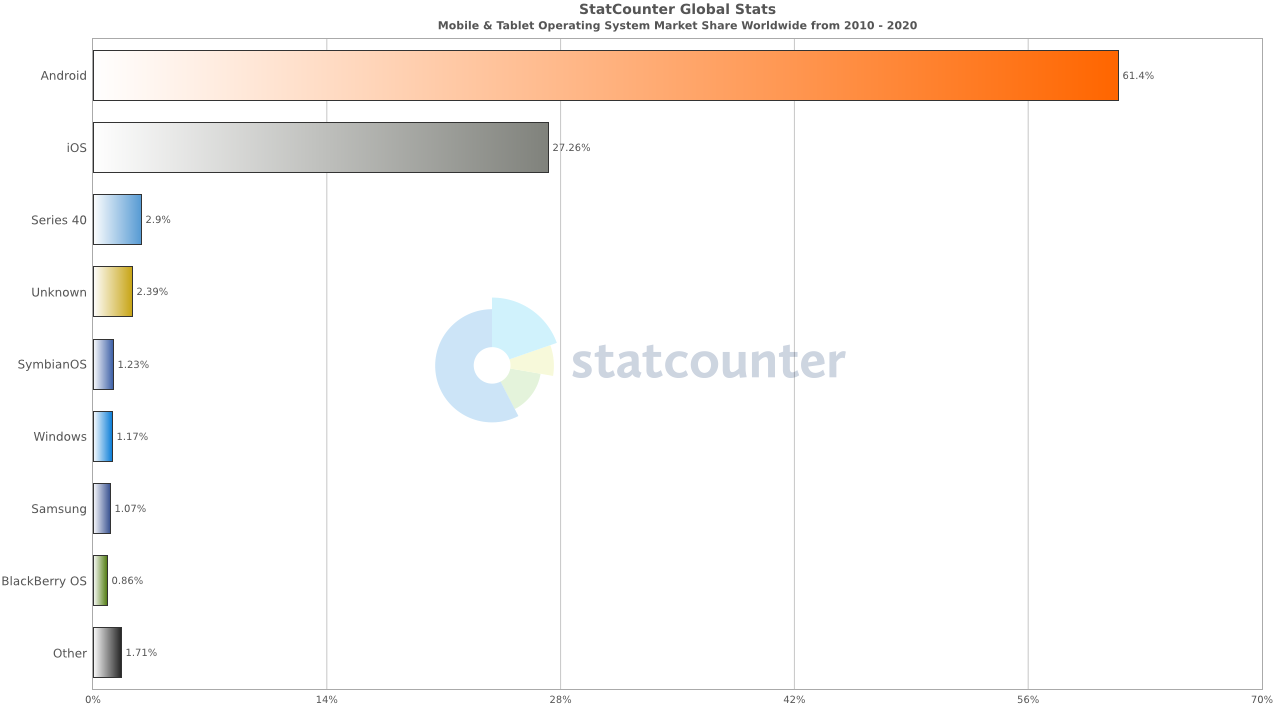
\includegraphics[width=.9\textwidth]{android_chart.png}
      \caption{Wykres udziału w rynku poszczególnych mobilnych systemów operacyjnych na przestrzeni 12 lat}
      \label{fig:android}
    \end{figure}
    Łatwa dostępność, ilość urządzeń na których jest on zainstalowany, szeroki wachlarz
    możliwości - te cechy napędzały ambicje twórców aplikacji mobilnych. Zaoferowany
    przez firmę Google Play Store, w przeciwieństwie do App Store pozwala na darmowe
    udostępnienie produktów o ile spełniają one odpowiednie warunki.

    Wraz z tak prężnym rozwojem rynku smartphone'ów, rozpoczęła się zmiana trendów.
    I o ile od początku XXI wieku światem królowały komputery, oferujące cały zasób 
    możliwości od nauki, po rozrywkę, tak smartphony z roku na rok coraz bardziej 
    zaczęły przypominać swoich stacjonarnych braci. 
    \begin{figure}[H]
      \centering
      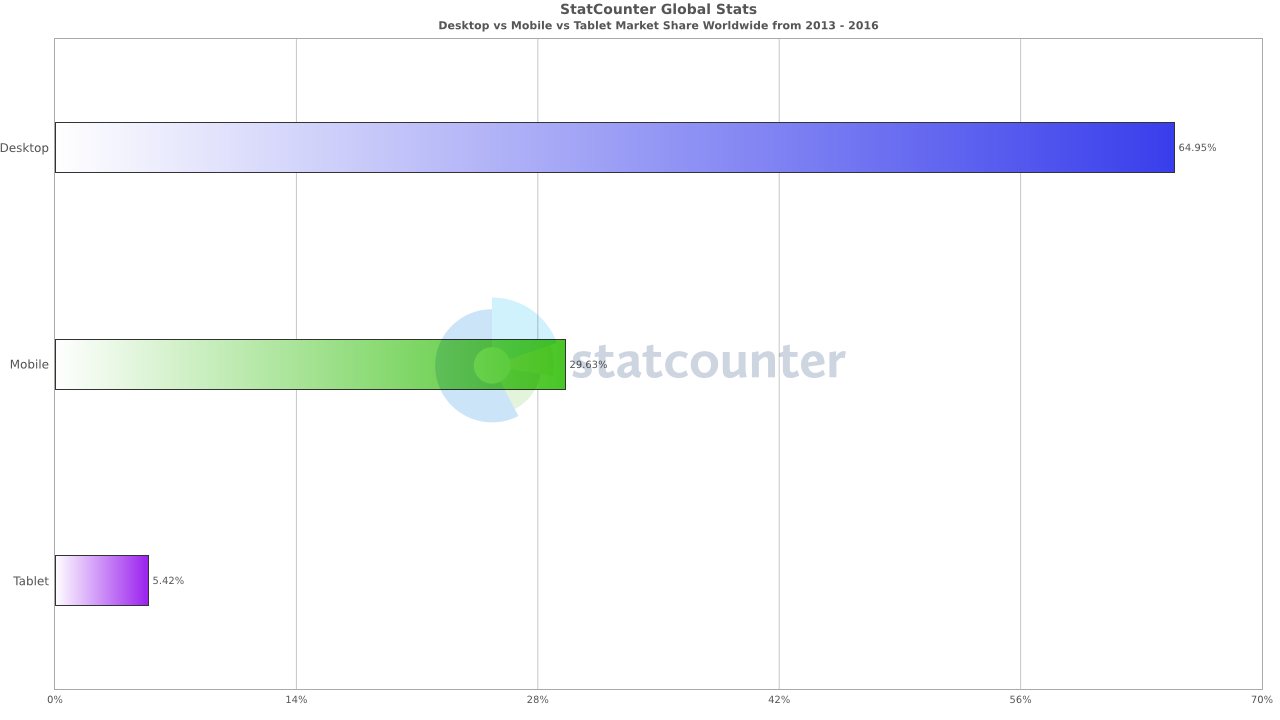
\includegraphics[width=.9\textwidth]{systems_chart1.png}
      \caption{Komputery, a smartphony na przestrzeni lat 2013-2016}
      \label{fig:2013}
    \end{figure} 
    \begin{figure}[H]
      \centering
      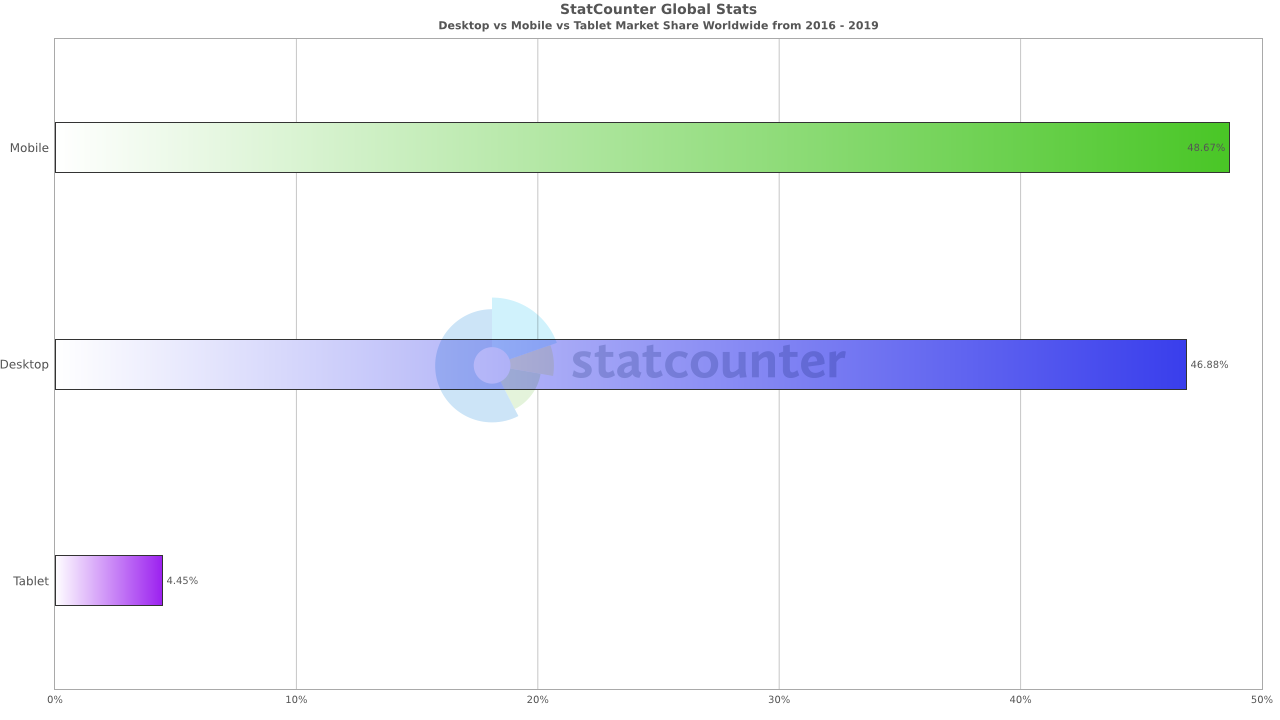
\includegraphics[width=.9\textwidth]{systems_chart2.png}
      \caption{Komputery, a smartphony na przestrzeni lat 2016-2019}
      \label{fig:2016}
    \end{figure} 
    Jednak urządzenia mobilne były i są w stanie zaoferować dużą większą wygodę 
    użytkowania, przenośność, oraz system znacznie łatwiejszy do przyswojenia dla 
    przeciętnego człowieka, nie wymagający szczególnej wiedzy do poprawnego
    zarządzania. Stąd u młodzieży umiejętności obsługi komputerów stacjonarnych
    zaczęła zanikać, jako że przestaje ona być tak kluczowa jak była jeszcze 10 lat
    temu. Jak podaje strona Broadbandsearch \cite{dvm}, już w 2016 roku większość "ruchu"
    internetowego była spowodowana przez urządzenia mobilne, bo aż 51.3\%, i po 
    rok 2021 oscyluje stabilnie w granicach 52\%. Jak podaje ten sam portal,
    różnice pomiędzy rokiem 2013, a 2019 w ilości czasu spędzanego dziennie na 
    użytkowaniu smartphonów i desktopów wygląda następująco:
    \begin{itemize}
      \item Średni czas użytkowania komputerów/laptopów spadł ze 144 minut dziennie, do 128 minut
      \item Średni czas użytkowania urządzeń mobilnych wzrósł z 88 minut, do średnio 203 minut dziennie 
    \end{itemize} 
    Takie wyniki sprawiły, że coraz więcej firm musiało zacząć liczyć się z 
    rynkiem urządzeń mobilnych, a obecnie częstą praktyką przy tworzeniu aplikacji 
    przeznaczonych zarówno na komputery stacjonarne, jak i smartphony, lub przy 
    pisaniu stron internetowych, jest stylizowanie ich najpierw na mniejsze ekrany,
    a następnie dostosowywanie pod urządzenia desktopowe. W przypadku marketingu, 
    zamiast "optymalizować" go pod kątem urządzeń mobilnych, zaczęto tworzyć zupełnie
    oddzielne kampanie marketingowe zarówno dla desktopów jak i smartphone'ów
    \cite{mobile_strategy}.
  }
  \subsection{Programowanie aplikacji na urządzenia mobilne}
  {
    Proces tworzenia aplikacji na systemy mobilne jest w dużym stopniu podobny do
    ich desktopowych odpowiedników. Projektując taką aplikację, należy początkowo wziąć
    pod uwagę rodzaj systemu operacyjnego, na którym ma ona działać, gdyż różne systemy
    mają swoje własne wymagania. To przekłada się często na fakt, że jedna aplikacja musi
    zostać w większości przepisana, aby spełniać warunki narzucane przez różne OS.
    Moc obliczeniowa jest kolejnym ważnym czynnikiem branym pod uwagę przy tworzeniu
    takiej aplikacji, gdyż o ile sprzęt dostępny w komputerach pozwala na wydajne
    działanie skomplikowanych systemów, tak smartphone'owy hardware, pomimo ogromnego
    postępu, ze względu na swoje rozmiary nadal jest ograniczony, stąd prostota i
    wydajność aplikacji są kluczowe dla bezproblemowego jej użytkowania.\\
    Obecnie rynek aplikacji mobilnych jest relatywnie młody, dlatego w przyszłości
    można oczekiwać, że powstanie język programowania / środowisko programistyczne
    unifikujące tworzenie aplikacji zarówno desktopowych, jak i mobilnych, jednak do
    czasu powstania takiego systemu, programiści muszą samodzielnie dostosowywać wygląd
    swoich projektów pod smartphony. Nie tylko rozmiar ekranu ma znaczenie, ale
    także współczynnik proporcji (z ang. Aspect Ratio), lub fakt, że urządzenia mobilne
    mają wbudowany akcelerometr pozwalający na obrócenie ekranu o \ang{90}. Wiele aplikacji
    pisanych jest tak, aby wyświetlane były w odpowiednim dla wizji programisty współczynniku
    proporcji, jednak większość tworzona jest zgodnie ze standardem przemysłowym,
    który dla urządzeń desktopowych wynosi 16:9, a dla mobilnych 9:16. Fakt ten, oraz
    rozmiary ekranu nie pozwalają na stworzenie jednolitego interfejsu dla obu typu
    urządzeń, stąd jedna aplikacja może wyglądać zupełnie inaczej w zależności od
    używanej platformy.\\
    Ostatnim ważnym czynnikiem wyróżniającym proces tworzenia aplikacji mobilnej, jest
    sposób jej testowania. Dla komputerów stacjonarnych, programiści zazwyczaj mają
    dostęp do platformy na którą przeznaczyć chcą swój produkt, przykładowo przy
    pisaniu aplikacji web'owej, działanie jej testuje się w przeglądarce. W przypadku
    aplikacji mobilnych, używa się specjalnych emulatorów, na których instaluje się
    swoje oprogramowanie, a następnie na bieżąco sprawdza jego działanie. Z jednej
    strony, pozwala to na szybkie, bezpieczne i wygodne testowanie, jednak emulatory te
    nie są w pełni poprawną symulacją prawdziwego systemu, więc często nie jest to
    możliwe, aby sprawdzić wszystkie możliwe, zaawansowane interakcje użytkownika.
  }
  \subsection{Speech to text}
  {
    Popularną opinią jest, iż lenistwo idzie w parze z ludzkim rozwojem 
    technologicznym. Wiele przypadków potwierdza tą regułę, sam Bill Gates, założyciel
    firmy Microsoft powiedział:\\ 
    “I choose a lazy person to do a hard job. 
    Because a lazy person will find an easy way to do it.”
    W duchu tych słów, ludzie jako rasa mają w zwyczaju być leniwymi, dlatego
    naturalną rzeczą stał się fakt, iż pisanie na klawiaturze nie jest najbardziej 
    optymalną techniką "porozumiewania się" z maszynami.
    
    W roku 1952, Bell Laboratories stworzyło system "Audrey", który był w stanie 
    rozpoznać wypowiedziane pojedyńcze cyfry, a 10 lat później, "Shoebox" od IBM
    mógł zrozumieć i odpowiedzieć na 16 słówek w języku Angielskim \cite{speech_history}.
    W latach siedemdziesiątych XX wieku, Amerykański Departament Obrony rozpoczął
    projekt o nazwie "SUR" - The Speech Understanding Research, którego owocem
    był "Harpy", system będący w stanie rozpoznać 1000 słów. Współzawodnictwo wielu
    firm w zakresie rozpoznawania mowy doprowadzało do powstawania dużej ilości nowych
    modeli, oraz metod, jeszcze bardziej optymalizujących cały proces.

    Do roku 2001, estymowana dokładność systemów rozpoznawania mowy wynosiła około 80\%,
    i przez dłuższy nie zostały osiągnięte godne uwagi postępy. Sytuacja jednak
    zmieniła się dzięki firmie Google, która uaktywniła w roku 2012 usługę Google 
    Voice Search. Okazała się ona być ogromnym sukcesem, jako że była to darmowa 
    aplikacja dostępna na urządzeniach mobilnych, stąd dzięki jej szerokiej dostępności,
    firma miała okazję zebrać dane pochodzące od milionów użytkowników, co przełożyło
    się bezpośrednio na poprawę dokładności algorytmu. Z czasem kolejne firmy
    zaczęły inwestować w technologię, a okres od roku 2010 do 2020 jest uważany za
    szczególnie ważny dla historii technologii rozpoznawania mowy. Tak oto w roku 2021
    użytkownicy mają dostęp do:
    \begin{itemize}
      \item Google Voice Search / Google Assistant - Google 
      \item Siri - Apple
      \item Cortana - Microsoft
      \item Alexa - Amazon
      \item I wiele innych ...
    \end{itemize}
    Firmy te prześcigają się o tytuł dokładności rozpoznawania mowy. W roku 2016, IBM
    osiągnęło wartość błędu 6,9\%. W 2017, Microsoft udało się osiągnąć błąd o
    wartości 5,9\%, jednak IBM szybko kontratakowało swoim 5,5\%. Firmy te
    nadal pozostają w tyle przy Google, którego błąd w 2017 roku osiągnął 4,9\% i do
    dziś pozostaje najdokładniejszym systemem rozpoznawania mowy dostępnym na rynku.
    Wraz z upływem czasu, technologia ta stawać się będzie coraz szybsza i
    efektywniejsza i bardzo możliwe jest, iż stanie się ona głównym interfejsem służącym
    komunikacji pomiędzy człowiekiem, a maszyną. 

    Przez większą część historii technologii "Speech Recognition", 
    najpopularniejszą metodą był HMM - "Hidden Markov Model" \cite{markov_article},
    opracowany już w latach osiemdziesiątych. W dużym skrócie, zamiast używania 
    słów i szukania w nich dźwiękowego wzorca, ma on za zadanie przewidzieć
    prawdopodobieństwo tego, że nieznane dźwięki mogą być słowami.\\   
    Proces analizy rozpoczyna się od zebrania informacji dźwiękowej,
    zwykle przy użyciu mikrofonu, i już na tym stadium pojawiają się pierwsze 
    problemy, takie jak:
    \begin{itemize}
      \item wyłapanie odpowiednich słów spośród dźwięków tła - szumu samochodów na 
      ulicy, lub inne osoby rozmawiające w bliskiej odległości.
      \item w przypadku szybko mówiącego rozmówcy, rozróżnienie w którym momencie
      wypowiedzi słowa kończą się, oraz kiedy zaczynają się kolejne.
      \item rozróżnianie różnych akcentów i sposobów mówienia pojedynczych jednostek,
      na przykład to samo zdanie wypowiedziane przez 10 letnią dziewczynkę, brzmieć
      będzie zupełnie inaczej, wypowiedziane przez 70 letniego mężczyznę. 
      \item odróżnianie homofonów - słów wymawianych w ten sam sposób, ale mających
      inne znaczenie
      \item poprawne zinterpretowanie zdań brzmiących w bardzo podobny sposób, ale
      oznaczających zupełnie różne rzeczy
    \end{itemize} 
    Dodatkowo, różne języki mają różną gramatyczną strukturę, co dodatkowo utrudnia
    stworzenie zunifikowanego systemu, zdolnego do przetwarzania wielu języków w 
    podobny sposób.\\
    Kolejnym krokiem jest przetworzenie zebranych danych na spektogram przy użyciu
    Szybkiej Transformaty Fouriera \cite{fourier}, oraz rozszczepienie
    rezultatu na mniejsze części, które poddawane są analizie mającej na celu
    określenie w jakich momentach znajdują się słowa. Następnie każde z nich są
    porównywane pod względem fonetycznego brzmienia i w ten sposób program stara
    się przewidzieć dokładne słowo, wypowiedziane przez użytkownika.

    W dzisiejszych czasach, technologia rozpoznawania mowy w głównej mierze opiera
    się na algorytmach sztucznej inteligencji połączonych z HMM.
  }
  \subsection{Bazy danych i ich rodzaje}
  {
    Sam koncept baz danych jest starszy niż same komputery stacjonarne, przykładowo w
    postaci szafek kartotekowych znanych tak dobrze z filmów ukazujących dokumenty CIA,
    bądź FBI. Pierwsza baza danych została zbudowana w latach sześćdziesiątych XX wieku,
    jednak ich historia w postaci znanej obecnie rozpoczyna się dopiero w 1970 roku,
    gdy naukowiec Edgar F. Codd opublikował pracę zatytułowaną "A Relational Model of
    Data for Large Shared Banks". Przedstawiała ona nowy sposób modelowania danych,
    przy pomocy budowania połączonych ze sobą tabel, mogących przechować jednorazowo
    jakąkolwiek formę danych. W tych czasach ilość pamięci była droga, a relacyjna baza
    danych pozwalała na odpowiednie, efektywne nią zarządzanie. Przez następne dwie
    dekady, technologia ta prężnie się rozwijała, dominując rynek światowy, a język
    SQL (Structured Query Language) stał się standardem pozwalającym aplikacjom na
    dostęp do wszelkich danych, w ilości i postaci w jakiej potrzebowały.

    W roku 1977, Larry Ellison, Bob Miner i Ed Oates założyli firmę o nazwie Software
    Development Laboratories (SDL), której celem było stworzenie bazy danych kompatybilnej
    z relacyjnym systemem. W przeciągu następnych 5 lat spółka zmieniła swoją nazwę
    dwukrotnie, w 1979 na Reletional Software Inc (RSI), a ostatecznie na w 1982 na
    Oracle Systems Corporation, obecnie jednego z największych i najbardziej dochodowych
    dystrybutorów baz danych na świecie. Swoje oprogramowanie napisali w języku C, co
    dawało bardzo dobre rezultaty pod względem optymalizacyjnym i pozwalało na 
    przeniesienie go na dowolną platformę wspierającą C. Przez wiele lat, Oracle
    bezkonkurencyjnie dominowało rynek, jednak pod koniec lat osiemdziesiątych, pojawiła
    się nowy firma, chcąca przejąć nad nim kontrolę, a był to Microsoft, który stworzył
    bazę danych na system OS/2, zwaną SQL Server 1.0, a następnie zaprojektował jej port
    na Windows NT, który powoli stawał się najpopularniejszym systemem operacyjnym
    używanym w komputerach osobistych. Sprawiło to, że SQL Server zaczął przeistaczać
    się w najnowszy standard w małej i średniej wielkości firmach, a nowo opracowane
    środowiska programistyczne Visual Basic, a następnie .NET pozwalały na łatwą
    integrację baz danych do projektów. We wczesnych latach dziewięćdziesiątych, pojawiło
    się najnowsze rozwiązanie, które wpłynęło na rynek w jeszcze większym stopniu niż
    którykolwiek z jego poprzedników, przynajmniej w kontekście rynku online. Aby zwalczać
    dominację Microsoftu i jego ścisłą kontrolę nad kodem używanym w większości systemów
    komputerów stacjonarnych, został uformowany ruch open-source - otwartego, a co za tym
    idzie darmowego kodu źródłowego. W roku 1995 powstała pierwsza wersja MySQL, opracowana
    przez firmę fundującą cały projekt open-source - MySQL AB. Oprogramowanie to stało
    się pierwszą znaczącą bazą danych używaną w przypadku stron internetowych, do dziś
    wykorzystywaną przez firmy takie jak Google, Facebook, czy Twitter. Otwartość kodu
    pozwoliła twórcom stron na niezależność wobec spółek takich jak Oracle'a, czy Microsoft'u. 

    Relacyjne bazy danych zostały zaprojektowane w czasach poprzedzających popularność
    internetu i były przeznaczone do operowania na jednej maszynie. W przypadku, gdy
    przytłaczająca ilość danych wykraczała poza możliwości jednego urządzenia, jedynym
    sposobem było połączenie wielu serwerów w klastry, a to sprawiało że przeniesienie
    tradycyjnej bazy danych opartej na SQL i przeznaczonej do działania na pojedynczym
    serwerze, było zadaniem wyjątkowo skomplikowanym i często dającym złe rezultaty.
    Aby temu zaradzić, zaczęto przykładać uwagę do technologii istniejącej już w latach
    sześćdziesiątych, a która w 1998 roku została przemianowana na NoSQL (Not only SQL).
    Nie było to rozwiązanie perfekcyjne, gdyż nie posiadało wielu zalet relacyjnych baz
    danych, jednak było szybsze i znacznie lepiej skalowalne, cechy które w okresie po
    internetowej rewolucji WEB 2.0, gdy w bardzo szybkim tempie pojawiało się zapotrzebowanie
    na kolejne jednostki pamięci, były na wagę złota. Obecnie, coraz to większą popularność
    zaczynają pozyskiwać chmurowe (cloud database), oraz autonomiczne bazy danych
    (self-driving database).\\
    {\large \bfseries Najpopularniejsze rodzaje baz danych} \cite{oracle-db}
    \begin{itemize}
      \item Relacyjne bazy danych (Relational databases) - Rekordy w bazie zorganizowane
      są w postaci tabel posiadających wiersze i kolumny. Różne tabele mogą posiadać
      pomiędzy sobą związki pozwalające im na wspólną kooperację. 
      \item Obiektowe bazy danych (Object-oriented databases) - Dane są przechowywane w
      postaci obiektów, posiadających w sobie określone pola.
      \item Rozproszone bazy danych (Distributed databases) - Dane przechowywane mogą być
      w wielu plikach, na wielu urządzeniach, rozproszone w różnych sieciach.
      \item Nierelacyjne bazy danych (NoSQL databases) - Pozwala na przechowywanie i
      manipulowanie danymi, które nie są ustrukturyzowane, w przeciwieństwie do relacyjnych
      baz danych, które definiują jak skomponowane mają być dane dostarczone do bazy. Ich
      popularność rosła wprost proporcjonalnie do ilości aplikacji web-owych i ich
      złożoności.
      \item Grafowe bazy danych (Graph databases) - Bazy, gdzie związki pomiędzy
      danymi są równie ważne, co same dane.
      \item Bazy danych OLTP (Online Transaction Processing) - Szybkie, analityczne
      bazy danych, projektowane z myślą o dużej ilości transakcji wykonywanych pomiędzy
      wieloma użytkownikami. 
      \item Hurtownia danych (Data warehouses) - Baza zaprojektowana pod kątem
      szybkiej wymiany danych i ich analizy
      \item Wielomodelowa baza danych (Multi-model database) - Ich celem jest połączenie
      wielu typów modeli baz danych w jeden, zintegrowany back-end. Mogą dzięki temu
      pomieścić wiele typów danych.
      \item Autonomiczne bazy danych (Self-driving databases) - Najnowsze i najbardziej
      rewolucyjne bazy, oparte na chmurowych bazach danych, wykorzystujące uczenie
      maszynowe do zautomatyzowania nimi zarządzania.
    \end{itemize}

    Zdobywającymi coraz większą popularność systemami bazodanowymi są chmurowe bazy danych,
    które postaram opisać się w kolejnym rozdziale.
  }
  \subsection{Chmurowe bazy danych}
  {
    Ideą chmurowych baz danych jest zmniejszenie zapotrzebowania firm na zakup własnych
    "fizycznych" serwerów, a zamiast tego zaoferowanie im płatnego dostępu do maszyn
    wirtualnych, na których dana firma mogłaby postawić swoją bazę danych. Czym jednak
    są maszyny wirtualne? 
    
    W skrócie, jest to wirtualne środowisko, funkcjonujące jako
    komputer, którego komponenty takie jak procesor, pamięć i interfejs sieciowy
    znajdują się na fizycznym systemie. Możliwe jest jednoczesne istnienie wielu maszyn
    wirtualnych na jednym systemie, zwanym inaczej "hostem". Dzięki oprogramowaniu
    "hypervisor", możliwe jest odseparowanie fizycznej maszyny, od wirtualnej,
    co stwarza bezpieczne środowisko do pracy i w przypadku, gdyby przykładowo na
    maszynie wirtualnej znalazł się wirus, nie wpłynie on na pracę hosta, jego
    działanie będzie ograniczone jedynie w zakresie maszyny wirtualnej.

    Aby korzystać z możliwości oferowanych przez "chmurę", firma może zdecydować się
    na stworzenie własnej, prywatnej infrastruktury, lub skorzystanie z udostępnianych
    publicznie serwisów chmurowych. Do najpopularniejszych obecnie należą:
    \begin{itemize}
      \item AWS - Amazon Wev Services
      \item Google Cloud Platform
      \item Microsoft Azure
      \item IBM Cloud
      \item Oracle Cloud
    \end{itemize}
    Dużą zaletą serwisów chmurowych jest możliwość łatwego dostosowania ich pod własne
    potrzeby, przykładowo w przypadku zapotrzebowania na większą ilość pamięci, lub
    większą moc obliczeniową wystarczy zazwyczaj zapłacić więcej za abonament, a nie
    trzeba się przejmować rozbudowywaniem własnej infrastruktury, co zajęłoby znacznie
    więcej czasu.
  }
  \subsection{API}
  {
    W wielu przypadkach przy tworzeniu aplikacji, programiści muszą zawrzeć
    informacje, których samodzielne wypisanie i skatalogowanie mogłoby zająć
    więcej czasu, niż sam proces pisania oprogramowania. Pojawia się również
    pytanie po co to wszystko robić, skoro wcześniej zrobił to już ktoś inny i
    dał on dostęp do pożądanych funkcjonalności. Dodatkowo co jeśli dana aplikacja
    jest zależna od innej usługi, przykładowo w przypadku gdy programista chciałby
    mieć dostęp do aktualnej pogody w dowolnym rejonie na świecie? Napisanie algorytmu
    będącego w stanie stworzyć model pogodowy, poprzez komunikację ze stacjami,
    lub satelitami pogodowymi na całym świecie w celu zebrania, przetworzenia, i 
    przewidzenia warunków pogodowych brzmi jak wielki projekt sam w sobie.
    Z pomocą przychodzą API, czyli Application Programming Interface, mające za 
    zadanie nie tylko ułatwić programistom tworzenie aplikacji, ale także 
    umożliwić komunikację pomiędzy różnymi usługami. Czym w takim razie dokładnie jest API?

    W momencie gdy przeciętny użytkownik chciałby wejść na witrynę internetową 
    "www.facebook.com", aby sprawdzić swój profil, lub przeczytać wiadomości, 
    przeglądarka próbuje wysłać zapytanie do serwera firmy Facebook, z prośbą o
    przekazanie informacji o tym jak wygląda strona, oraz o dostosowanie jej pod
    konkretnego użytkownika. Serwer odsyła wtedy potrzebne informacje, które przeglądarka,
    znana inaczej jako "klient", jest w stanie zinterpretować, a następnie wyświetlić 
    pożądany przez użytkownika wynik. Dla klienta, serwer Facebook'a jest API, co oznacza,
    że za każdym razem gdy dana osoba chce wejść na jakąkolwiek stronę internetową,
    wchodzi ona w interakcję z API danego serwera, nie znaczy to jednak, że jest ono
    tożsame z samym serwerem. Jest to jedynie jego część, odpowiedzialna za przetwarzanie
    zapytań i wysyłanie odpowiedzi - pakietów informacji mogących przybrać rozmaite formy,
    w zależności od potrzeb.
    
    Istnieje wiele rodzajów API, mogą się dzielić na różne typy, ale także posiadać
    odmienne architektury. Głównymi typami API są:
    \begin{itemize}
      \item Open APIs - znane również jako API publiczne, są szeroko dostępne do użytku z
      minimalnymi ograniczeniami. Mogą być albo w pełni "otwarte", lub wymagać jedynie
      klucza API - ciągu znaków dzięki którym API będzie mogła zidentyfikować aplikację
      do której przesyłane będą dane.
      \item Internal APIs - w przeciwieństwie do Open APIs, są one "ukryte" i przeznaczone
      do użytku wewnątrz firm, w celu przekazywania zasobów pomiędzy zespołami danej spółki.
      \item Partner APIs - są one podobne do Open APIs, jednak dostęp do nich jest
      ograniczony, często wymagający opłaty.
      \item Composite APIs - typ, mający za zadanie dać dostęp do różnych serwisów i
      źródeł danych jednocześnie. Są one szczególnie użyteczne w architekturze
      mikroserwisowej \cite{microservices}, gdzie aby wykonać jedno zadanie, użytkownik
      może potrzebować informacji od paru serwisów jednocześnie. Używanie Composite APIs
      może zredukować obciążenie serwera i poprawić płynność działąnia aplikacji.
    \end{itemize}
    Architektury API mają za zadanie sprecyzować ograniczenia nakładane na różne 
    protokoły, definiujące zasady którymi należy się kierować przy wysyłaniu zapytań -
    jakie komendy należy użyć, oraz jakie typy danych są akceptowalne. Najpopularniejszymi
    architekturami i protokołami są:
    \begin{itemize}
      \item REST (Representational State Transfer) - w przeciwieństwie do innych 
      wymienionych nie jest protokołem. Kilkoma przykładowymi i najważniejszymi warunkami
      jakie powinien spełniać interfejs API RESTful korzystający z protokołu HTTP są
      \cite{rest}:
      \begin{itemize}
        \item Interfejsy API REST są oparte na zasobach — dowolnym obiekcie, danych lub 
        usłudze, które są dostępne dla klienta.
        \item Zasób ma identyfikator URI służący do unikatowej jego identyfikacji.
        \item Interakcja klientów z usługą odbywa się przez wymianę reprezentacji zasobów.
        Najczęściej używanym formatem wymiany danych jest notacja JSON.
        \item Interfejsy API REST korzystają z ujednoliconego interfejsu, co ułatwia 
        rozdzielenie implementacji klienta od implementacji usługi.
        \item Interfejsy API REST korzystają z bezstanowego modelu żądań. Żądania HTTP 
        powinny być niezależne i mogą występować w dowolnej kolejności, dlatego 
        zachowywanie informacji o stanie przejściowym między żądaniami nie jest możliwe.
        Informacje są przechowywane jedynie w zasobach, a każde żądanie powinno być 
        niepodzielną operacją.
        \item Interfejsy API REST są sterowane za pomocą hipermedialnych linków, 
        zawartych w reprezentacji.
      \end{itemize}
      \item JSON-RPC i XML-RPC (Remote Procedural Call Protocol) - żądanie może posiadać
      wiele parametrów, ale oczekiwać tylko jednego rezultatu. W przeciwieństwie do 
      architektury REST, nie działa na zasobach, ale na wywoływaniu odpowiednich metod,
      a identyfikator URI zamiast zasobu identyfikuje serwer, stąd nie przechowuje żadnych
      informacji w swoich parametrach. Oba protokoły różnią się od siebie jedynie notacją,
      za pomocą której są zakodowane wywołania.
      \item SOAP (Simple Object Access Protocol) - protokół oparty na notacji XML, używający
      do komunikacji protokołu HTTP. Został on zaprojektowany jako pośrednik, umożliwiający
      łatwą komunikację pomiędzy aplikacjami napisanymi w różnych językach programowania.
    \end{itemize} 
  }
  \subsection{Analiza konkurencyjnych rozwiązań}
  {
    Istnieje bardzo dużo aplikacji oferujących możliwość liczenia kalorii, jednak w 
    większości różnią się one jedynie szatą graficzną, oraz dostępem do funkcjonalności,
    których część jest nieczęsto niedostępna do darmowego użytkowania.
    \subsubsection{Fitatu}
    {
      Jest to aplikacja najprostsza w obsłudze z pozostałych rozwiązań, jako że stara się
      zawrzeć jak najwięcej informacji i funkcjonalności na głównej stronie co jednocześnie
      ułatwia jej użytkowanie, ale przekłada się na jej czytelność, ukazując duże ilości
      tekstu, co może przytłoczyć nowego użytkownika.
      \begin{figure}[H]
        \centering
        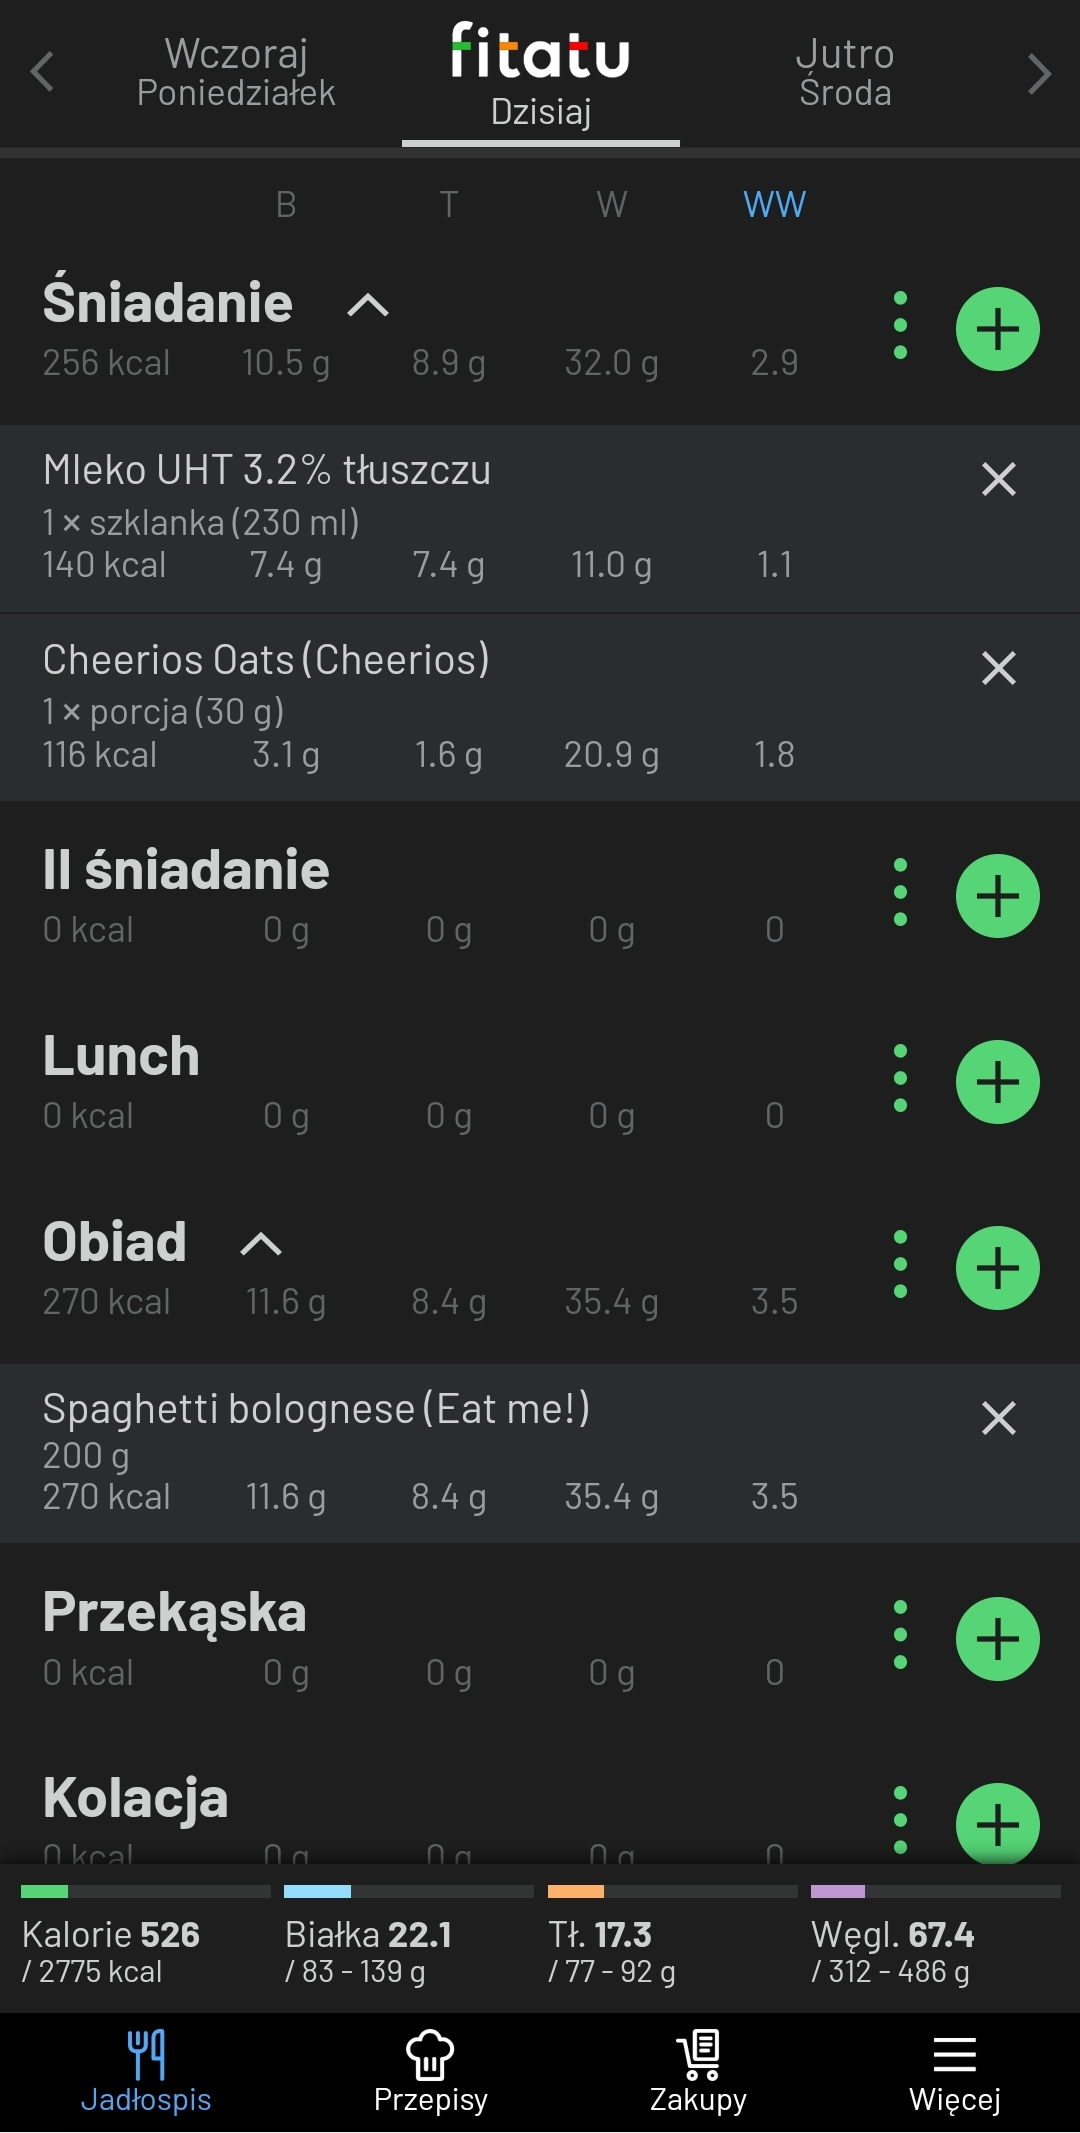
\includegraphics[width=.4\textwidth]{fitatu_pro_1.jpg}
        \caption{Fitatu - Ekran główny}
        \label{fig:fit1}
      \end{figure} 
      \begin{center}
        \begin{tabularx}{ \textwidth } {
          | >{\centering\arraybackslash}X
          | >{\centering\arraybackslash}X
          | }
         \hline
         \bfseries Zalety & \bfseries Wady \\
         \hline
         Rozpisanie najpopularniejszych posiłków jednego pod drugim, co ułatwia
         rozplanowanie kolejnych dań & 
         Bardzo duży rozmiar banerów informacyjnych, zasłaniających większą część
         interfejsu \\
         \hline
         Menu aplikacji jest modyfikowalne, pozwala na określenie w których godzinach
         jest spożywany dany posiłek, oraz na łatwe zmodyfikowanie celów użytkownika. & 
         Mały rozmiar paska podsumowującego spożyte danego dnia wartości odżywcze \\
         \hline
         Aplikacja posiada bardzo dokładną listę najróżniejszych składników odżywczych,
         rozpisanych w bardzo przejrzysty sposób, co pozwala na niezwykle szczegółowe
         rozplanowanie diety & 
         Bliskie rozłożenie przycisków do dodawania posiłków, co przekłada się na
         mniejszy komfort użytkowania \\
         \hline
        \end{tabularx}
      \end{center}
      \begin{figure}[H]
        \centering
        \begin{subfigure}{.5\textwidth}
          \centering
          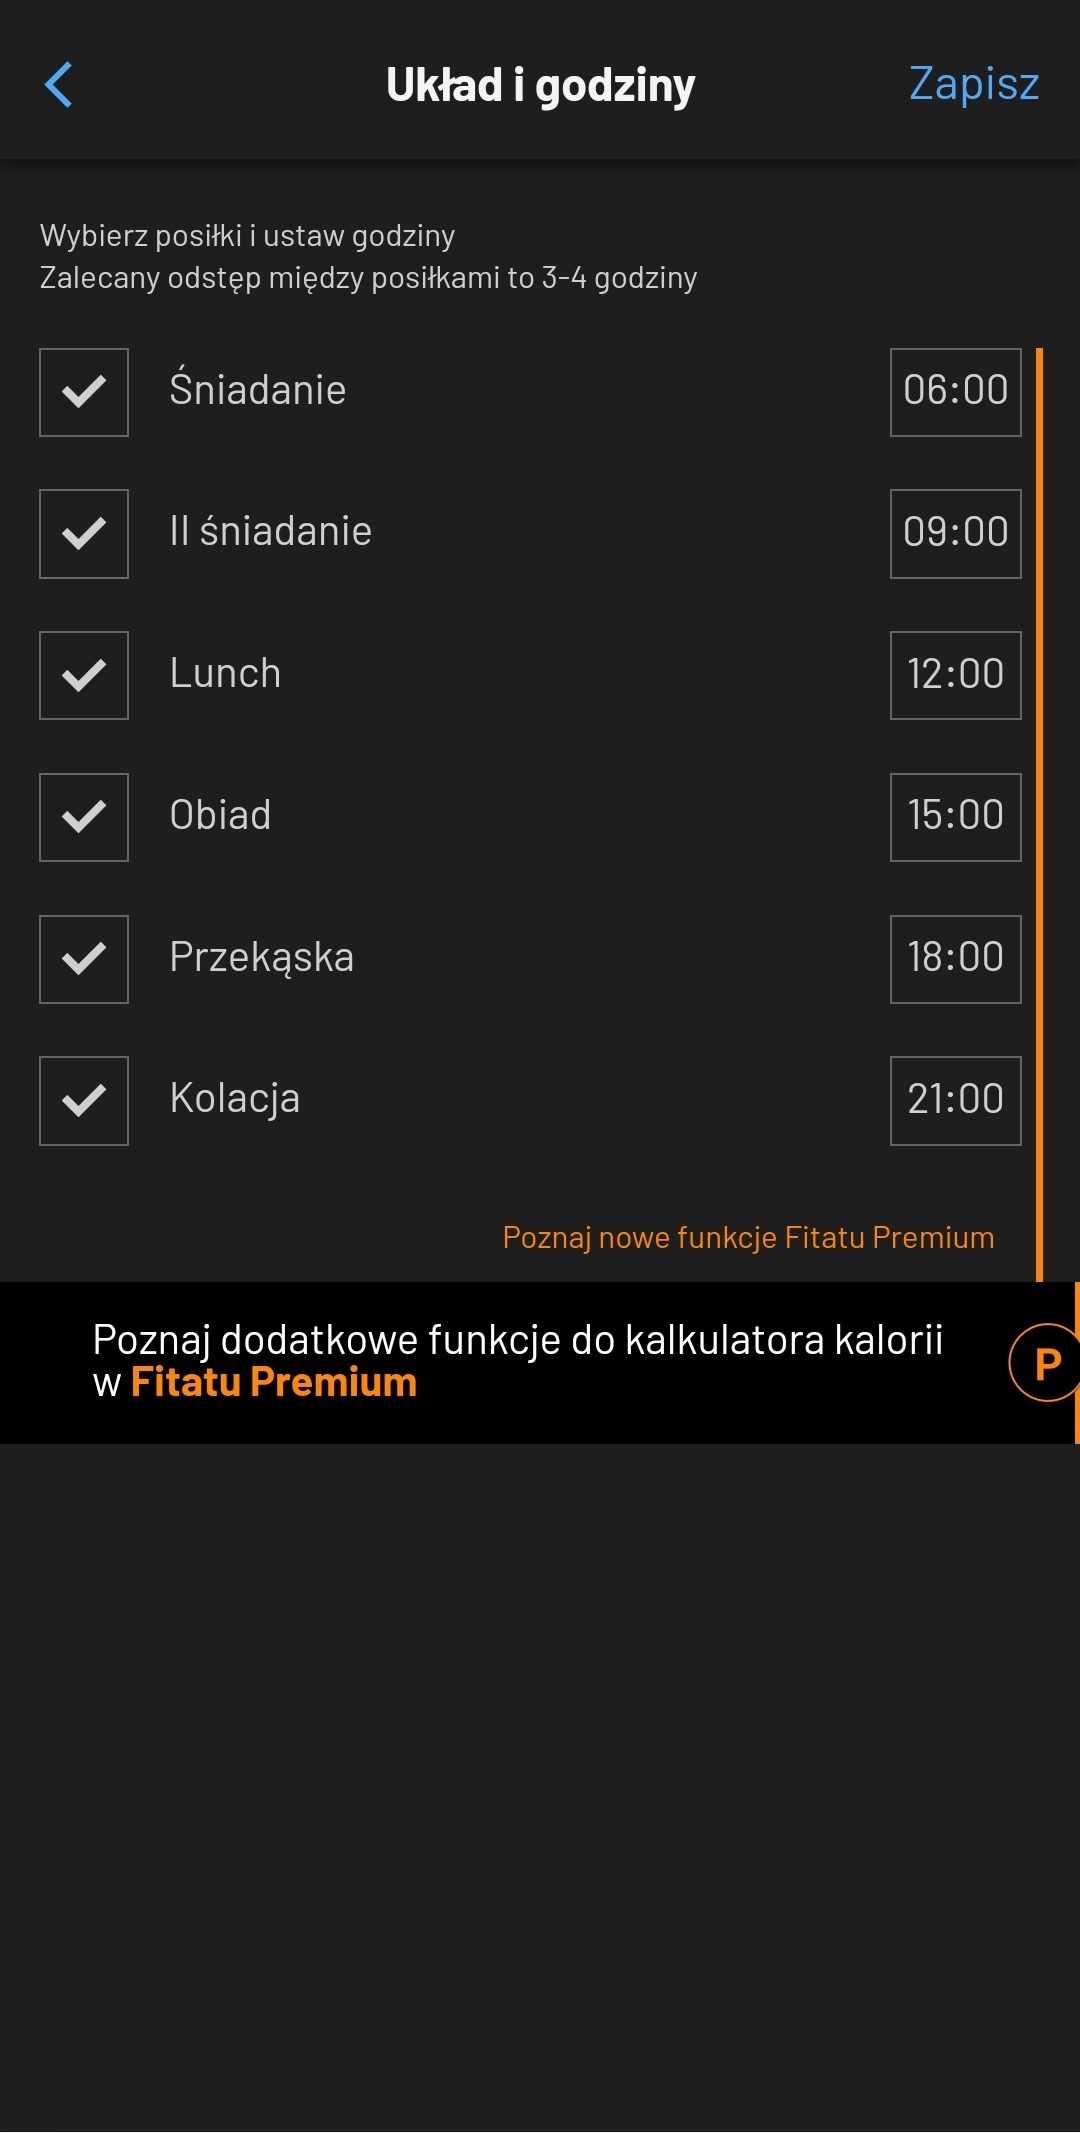
\includegraphics[width=.6\linewidth]{fitatu_pro_2.jpg}
          \caption{Ekran modyfikacji rozkładu dnia}
          \label{fig:subfit1}
        \end{subfigure}%
        \begin{subfigure}{.5\textwidth}
          \centering
          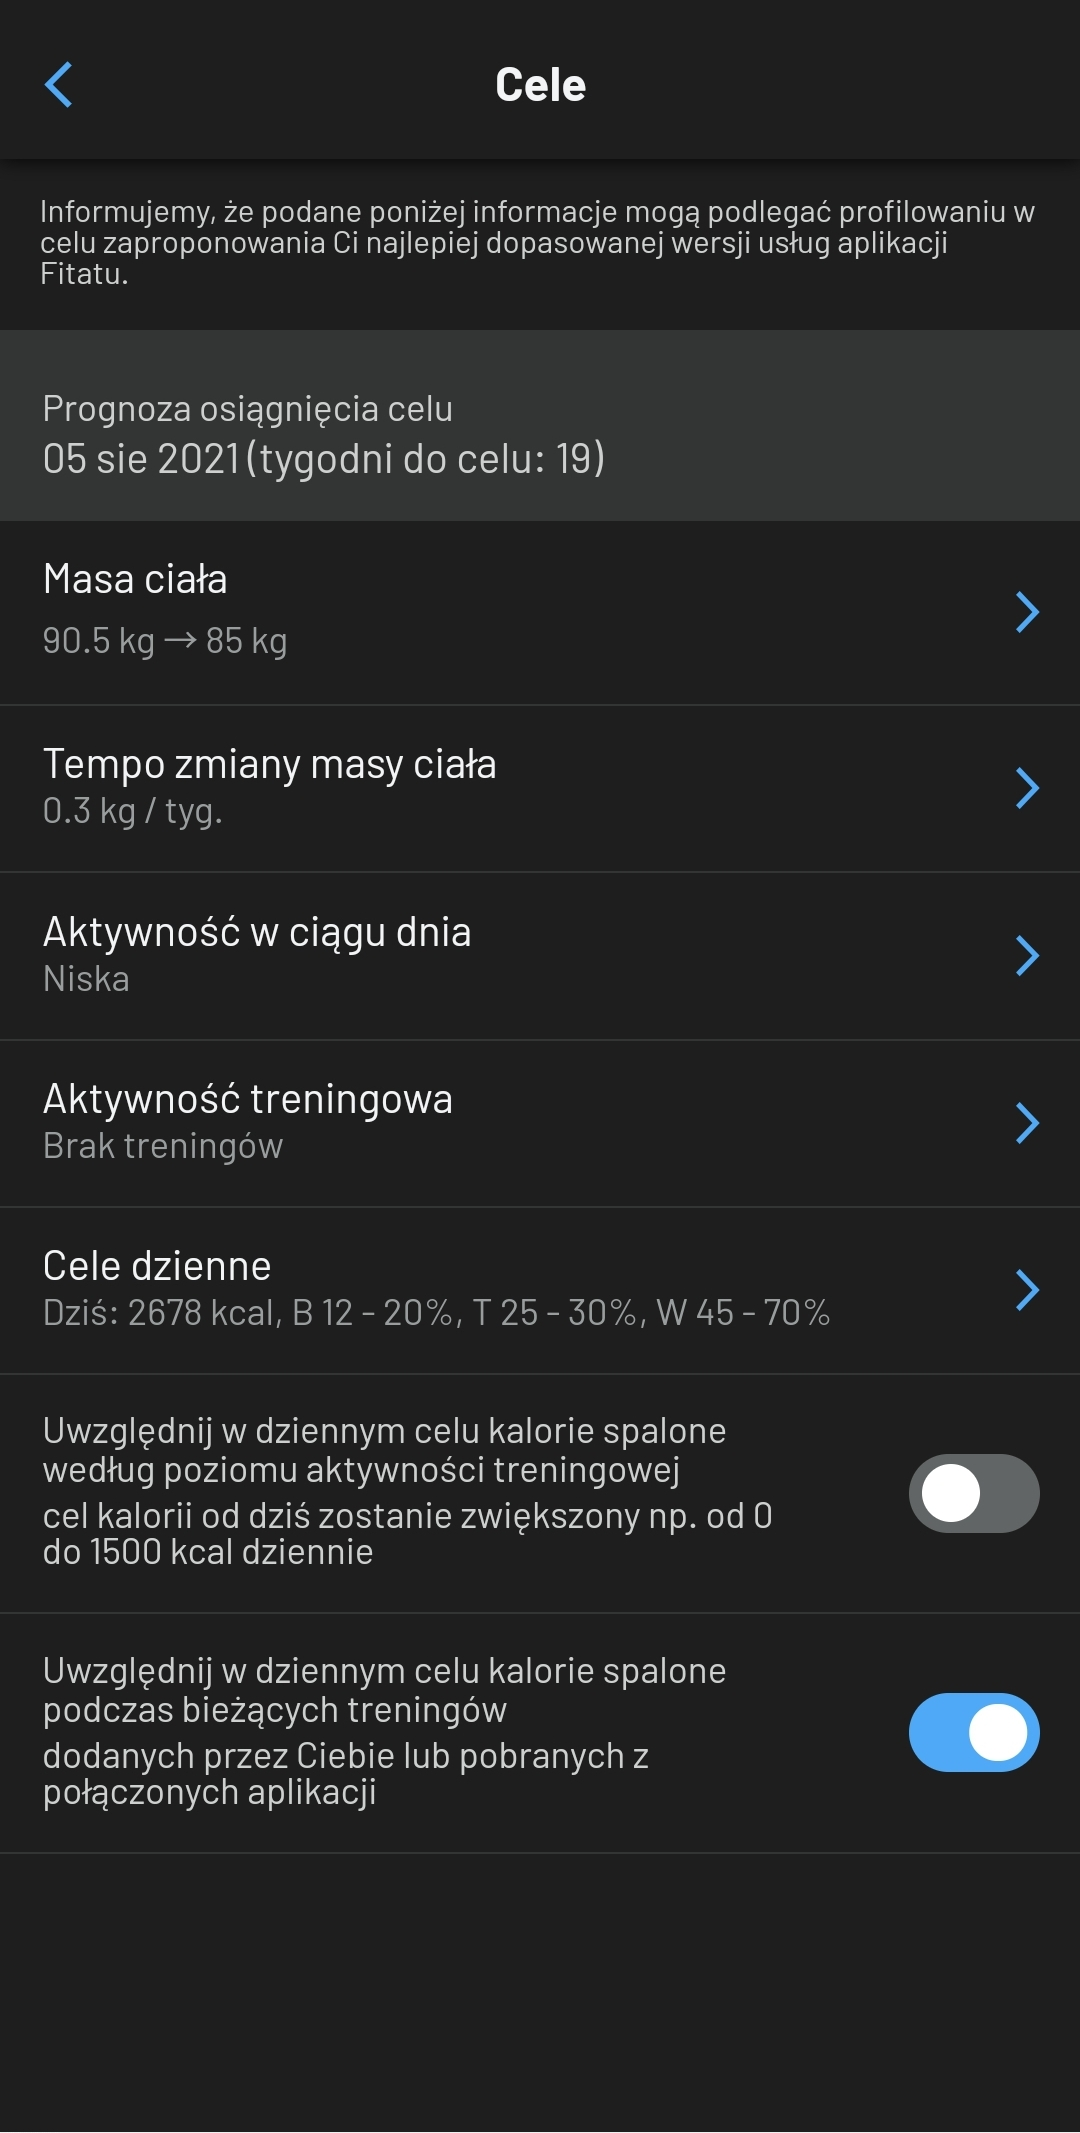
\includegraphics[width=.6\linewidth]{fitatu_pro_3.jpg}
          \caption{Ekran modyfikacji celów użytkownika}
          \label{fig:subfit2}
        \end{subfigure}
        \caption{Fitatu - Ekrany modyfikacji}
        \label{fig:fit2}
      \end{figure} 
        
      \begin{figure}[H]
        \centering
        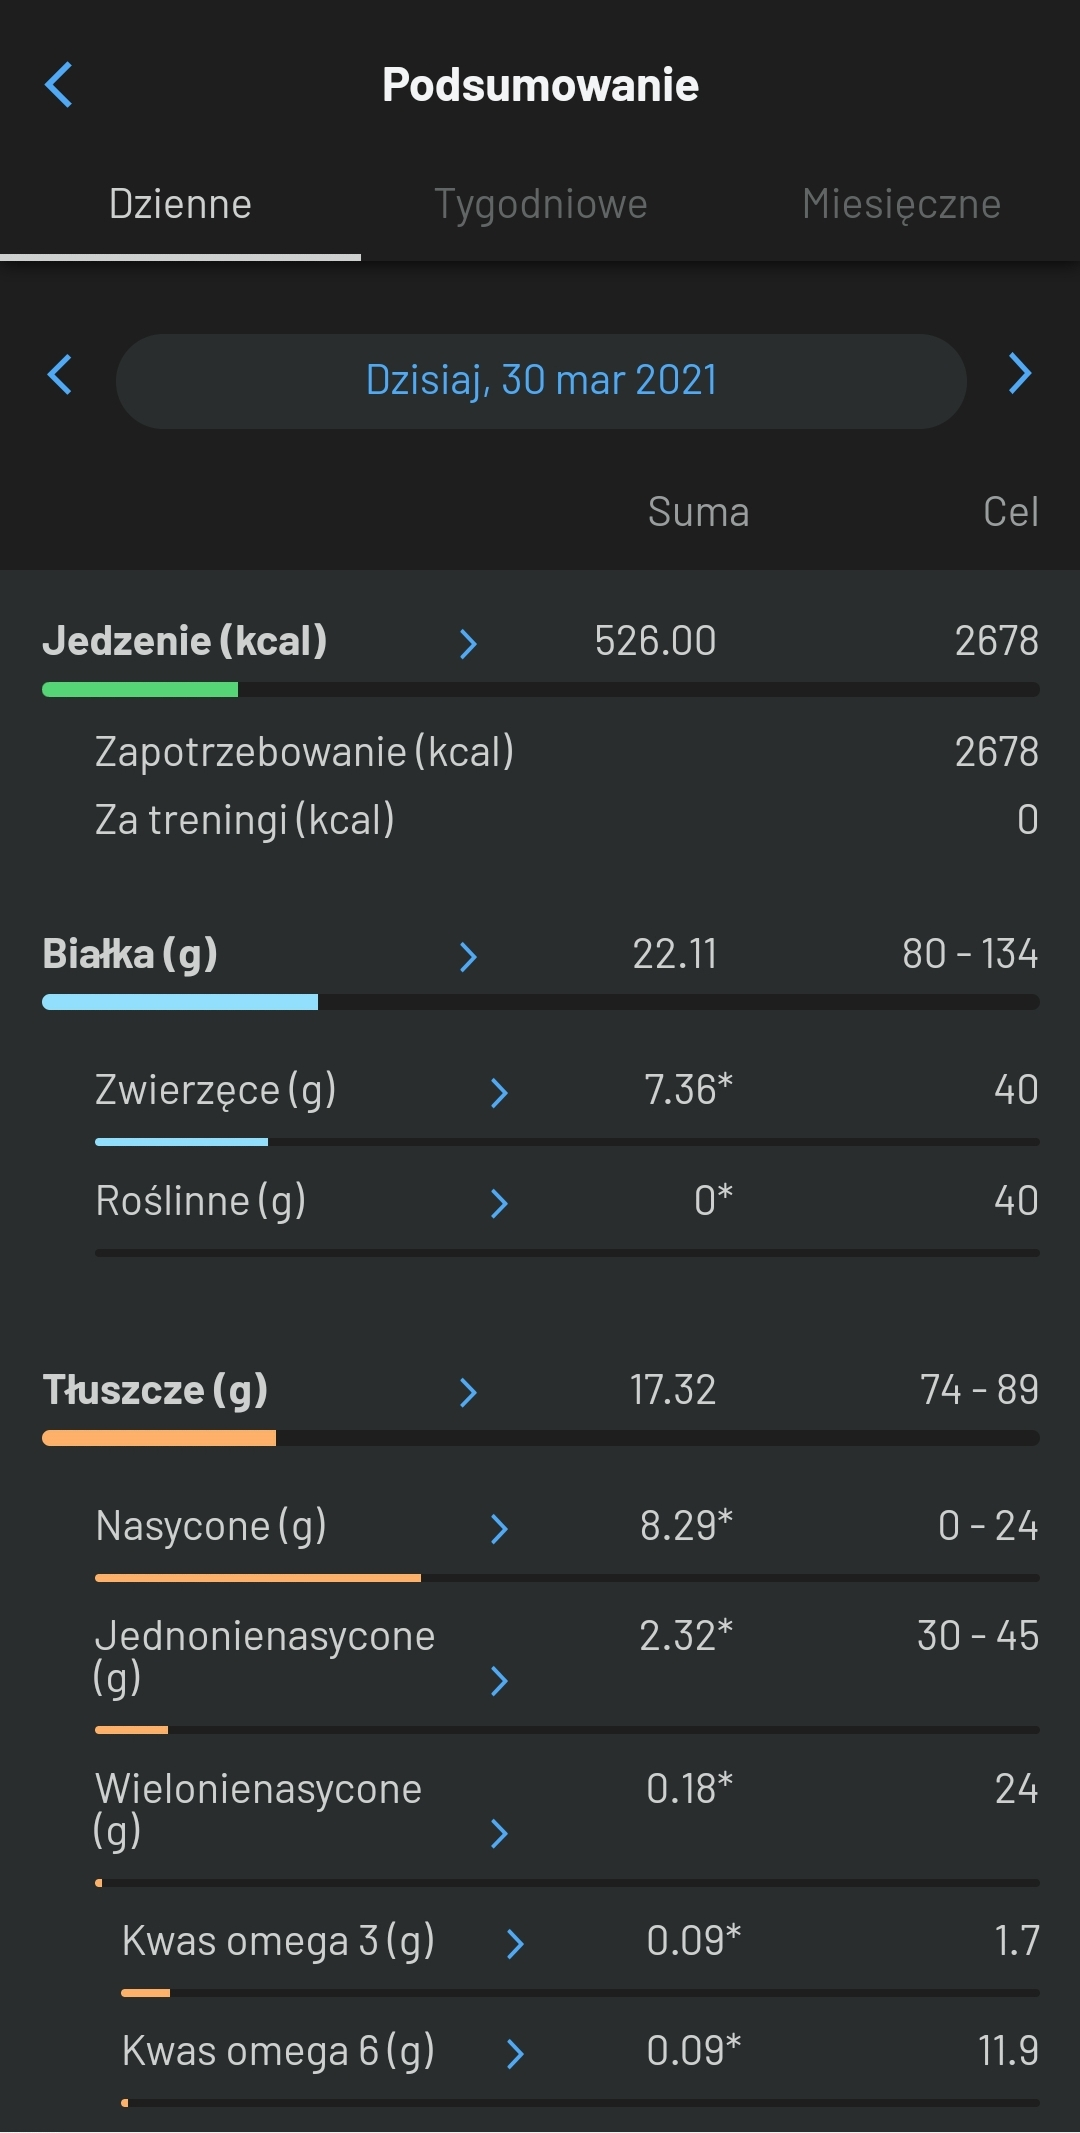
\includegraphics[width=.3\textwidth]{fitatu_pro_4.jpg}
        \caption{Fitatu - Ekran szczegółowego podsumowania}
        \label{fig:fit3}
      \end{figure} 
      
      \begin{figure}[H]
        \centering
        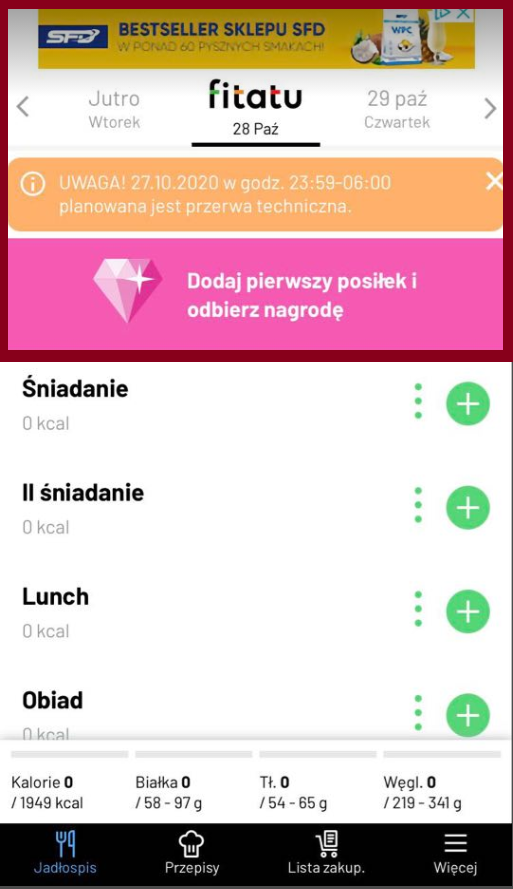
\includegraphics[width=.3\textwidth]{fitatu_con_1.png}
        \caption{Fitatu - Ekran zawierający banery informacyjne}
        \label{fig:fit4}
      \end{figure}
        
    }
    \subsubsection{Yazio}
    {
      Yazio jest aplikacją najbardziej ograniczoną pod względem funkcjonalności dostępnych
      w wersji darmowej, aby mieć dostęp do większości z nich należy posiadać płatną wersję
      PRO.\\
      Do zalet aplikacji należą:
      \begin{itemize}
        \item Duże pole podsumowujące dzień usytuowane na środku ekranu, w przejrzysty
        sposób prezentujące informacje o postępie danego dnia.
        \begin{figure}[H]
          \centering
          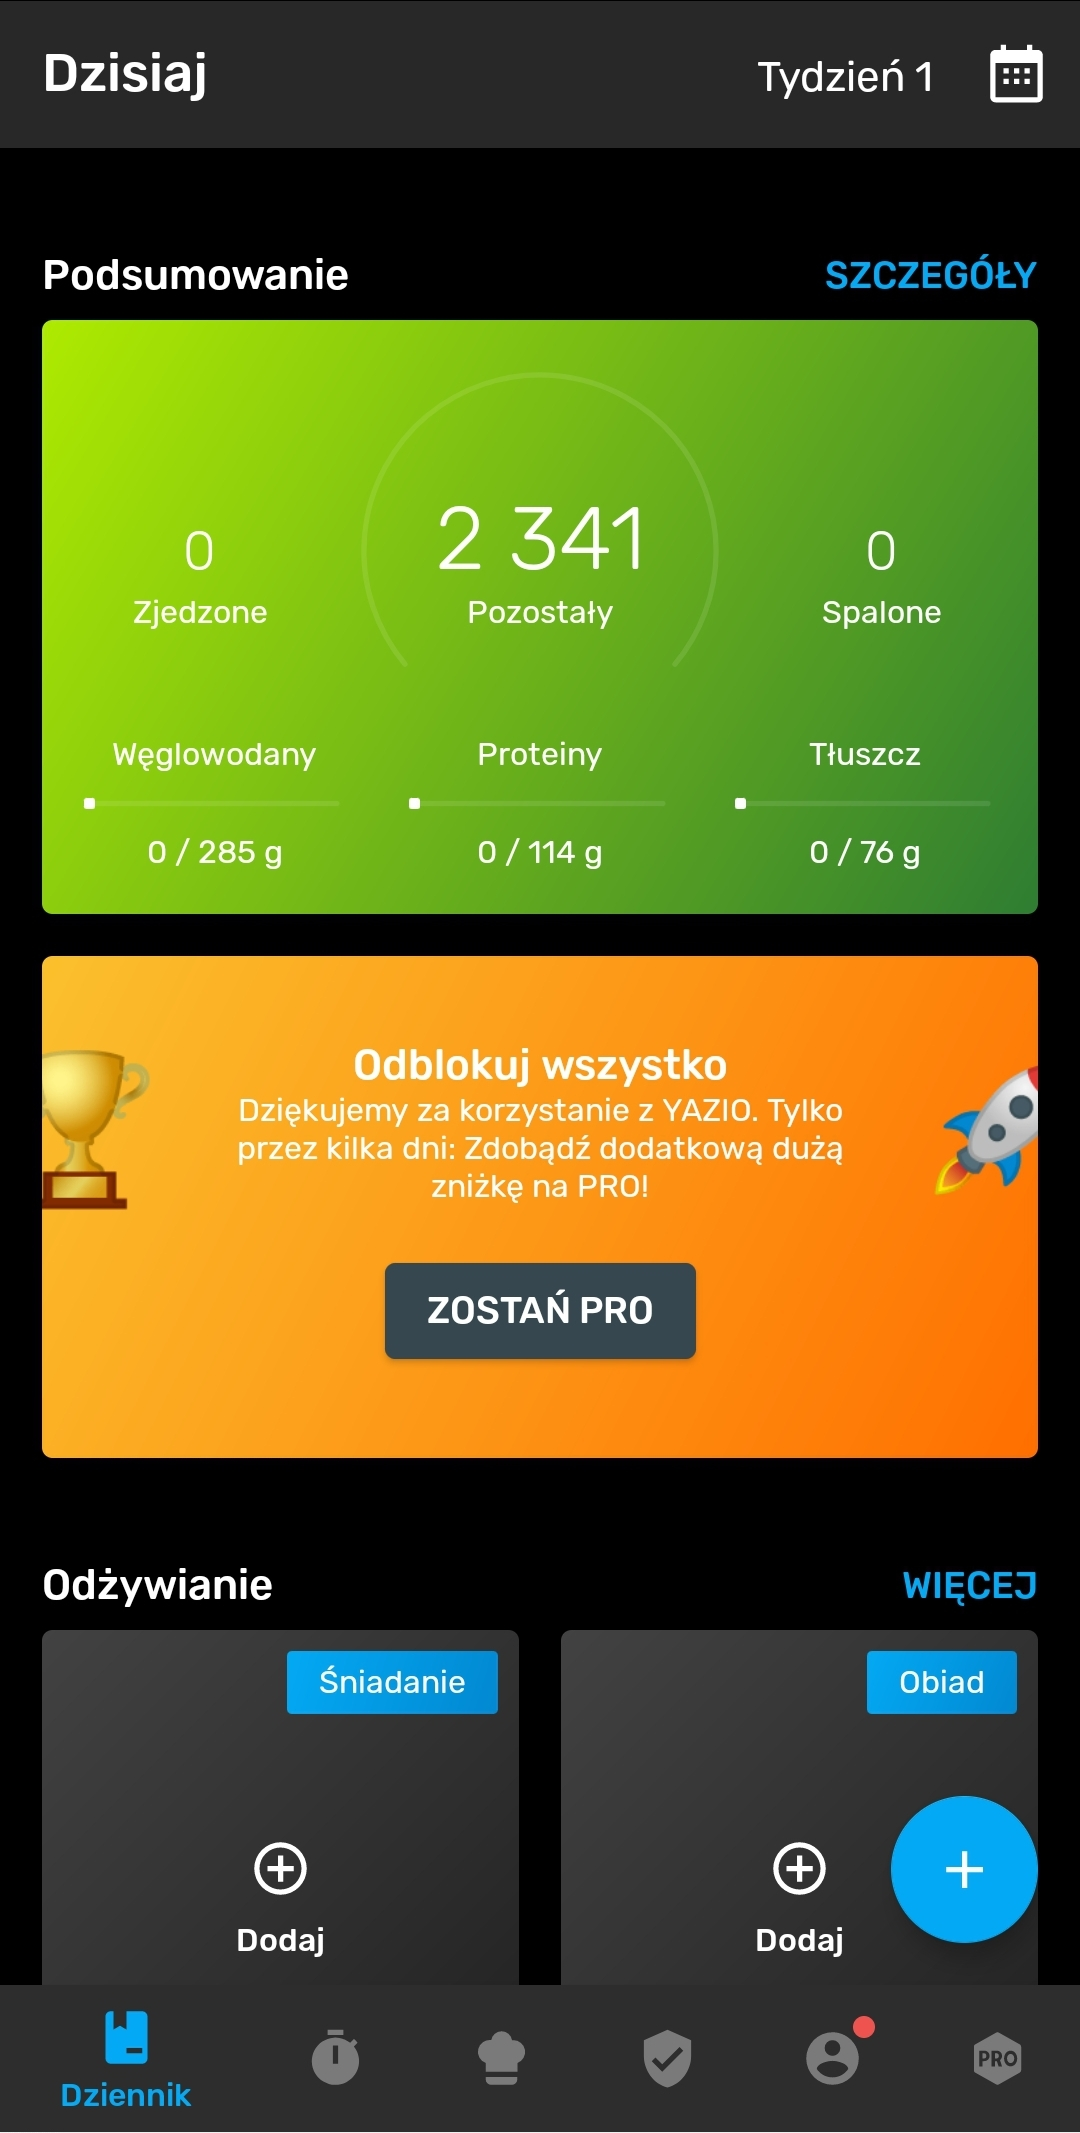
\includegraphics[width=.3\textwidth]{yazio_1.jpg}
          \caption{Yazio - Ekran główny}
          \label{fig:yaz1}
        \end{figure}
        \item Dodawanie jedzenia i interesujących użytkownika aktywności znajduje się pod
        jednym przyciskiem "+"
        \begin{figure}[H]
          \centering
          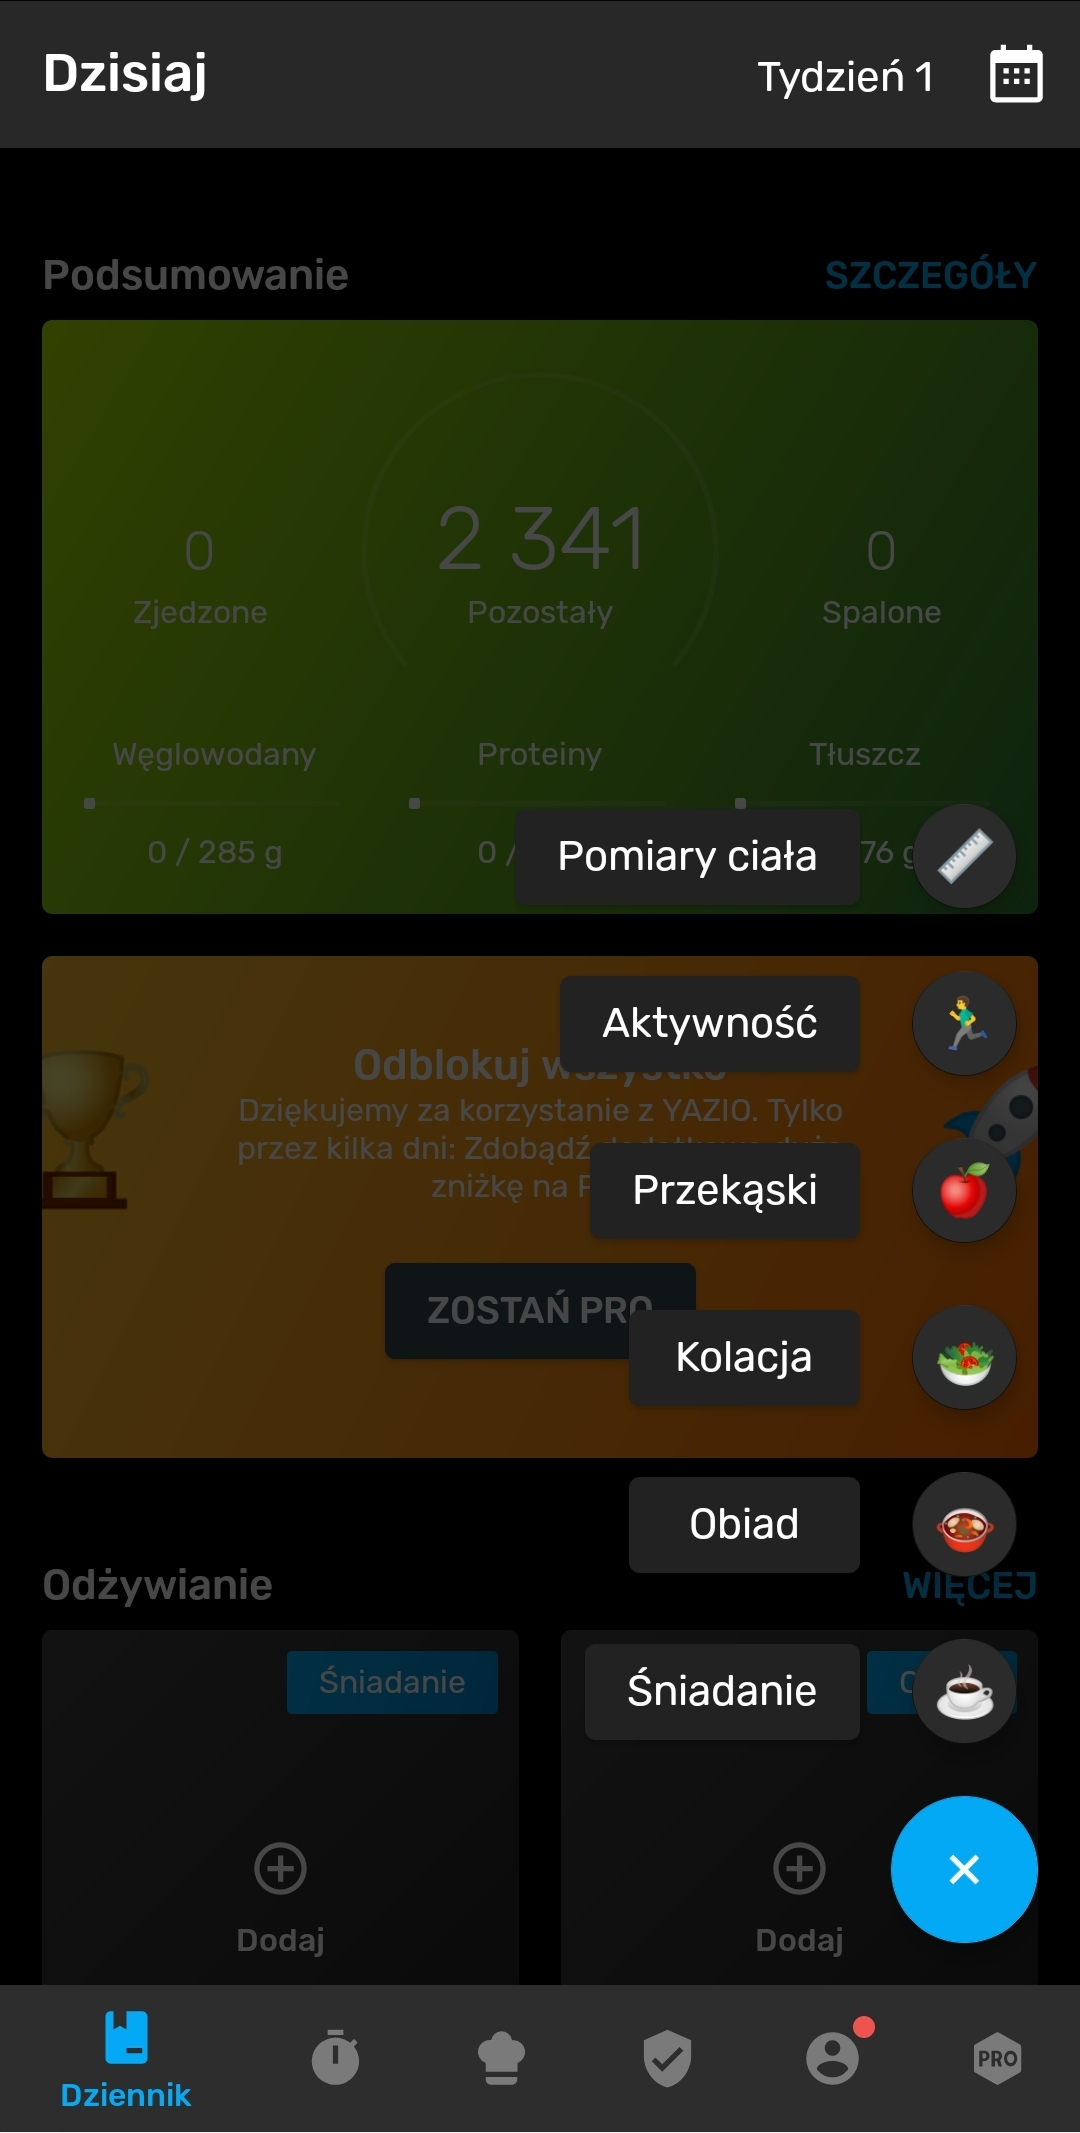
\includegraphics[width=.3\textwidth]{yazio_2.jpg}
          \caption{Yazio - Ekran z klikniętym przyciskiem "+"}
          \label{fig:yaz2}
        \end{figure}
      \end{itemize}
      Największą wadą aplikacji jest fakt jak bardzo ograniczona jest ona w wersji darmowej.
      W przypadku chęci sprawdzenia informacji o zjedzonych wartościach odżywczych, użytkownik
      ma dostęp jedynie do ilości zjedzonych kalorii, węglowodanów, protein, oraz tłuszczu,
      natomiast cała reszta, przykładowo witaminy nie są dostępne za darmo. 
      \begin{figure}[H]
        \centering
        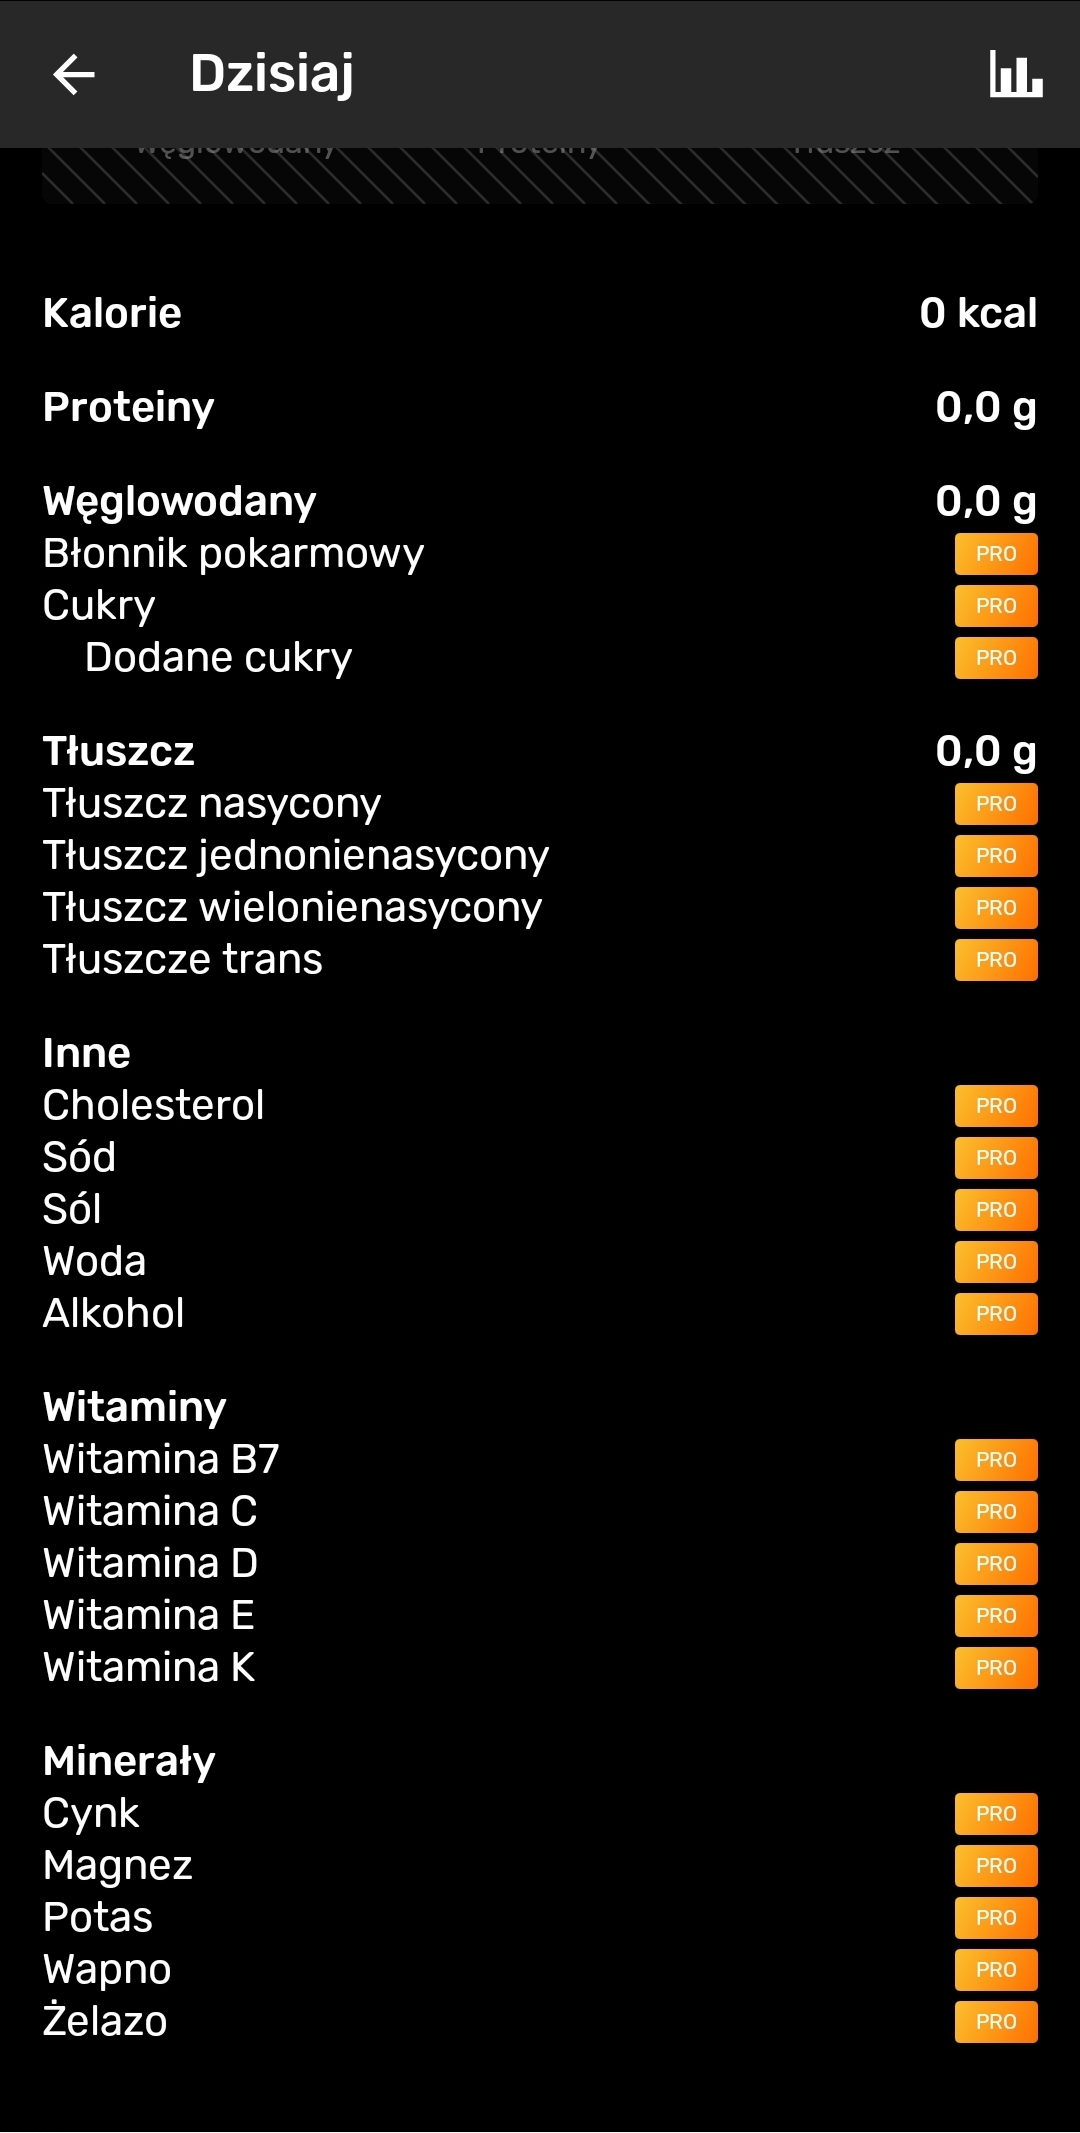
\includegraphics[width=.3\textwidth]{yazio_3.jpg}
        \caption{Yazio - Ekran podsumowujący}
        \label{fig:yaz3}
      \end{figure}
      Jeśli użytkownik nie chce inwestować pieniędzy, spośród konkurencji Yazio wypada 
      najgorzej.
    }
    \subsubsection{Fatsecret}
    {
      Pod względem wizualnym, Fatsecret łączy najlepsze cechy konkurencji, prezentując
      główny ekran podobny do Fitatu, jednak przedstawiony w sposób dużo bardziej 
      minimalistyczny, stąd czytelniejszy, a także posiadający ciekawie przedstawione 
      podsumowanie w postaci kwadratowej siatki, zapełnianej wraz z postępem zjedzonych posiłków.
      Nie jest to jednak rozwiązanie tak czytelne, jak przypadku aplikacji Yazio.
      \begin{figure}[H]
        \centering
        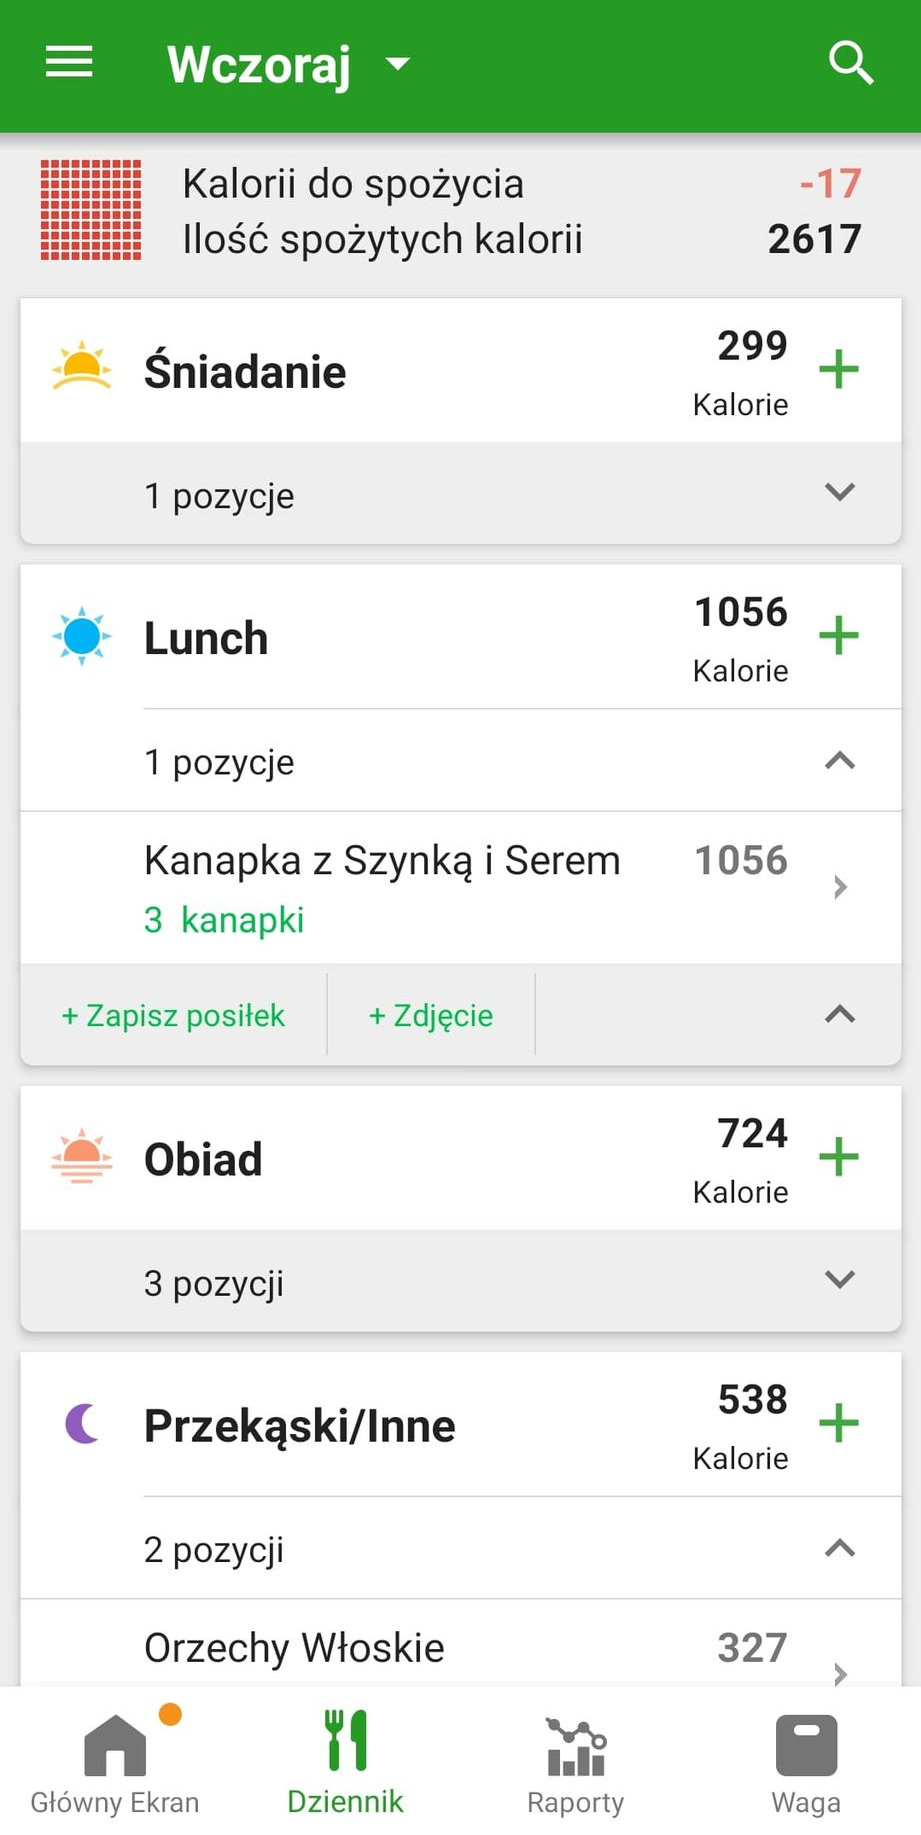
\includegraphics[width=.3\textwidth]{fatsecret_1.png}
        \caption{Fatsecret - Ekran główny}
        \label{fig:fat1}
      \end{figure} 
      
      \begin{center}
        \begin{tabularx}{ \textwidth } {
          | >{\centering\arraybackslash}X
          | >{\centering\arraybackslash}X
          | }
         \hline
         \bfseries Zalety & \bfseries Wady \\
         \hline
         Podobnie jak w przypadku Fitatu, rozpisanie najpopularniejszych posiłków
         jednego pod drugim, jednak w dużo czytelniejszy sposób & 
         Ilość wartości odżywczych, która jest mniej dokładna, niż w przypadku aplikacji 
         Fitatu, jednak zdecydowanie większa niż w bezpłatnej wersji Yazio \\
         \hline
         Menu podsumowujące znajdujące się tuż pod posiłkami i przedstawia dane w
         postaci aż dwóch różnych diagramów. & 
         Do odblokowania wszystkich funkcji aplikacja zmusza użytkowania do założenia
         konta. \\
         \hline
         Sekcja "Raporty" pozwala zobaczyć podsumowanie na przestrzeni dłuższego okresu
         czasu. &
          \\
         \hline
        \end{tabularx}
      \end{center}
      
      \begin{figure}[H]
        \centering
        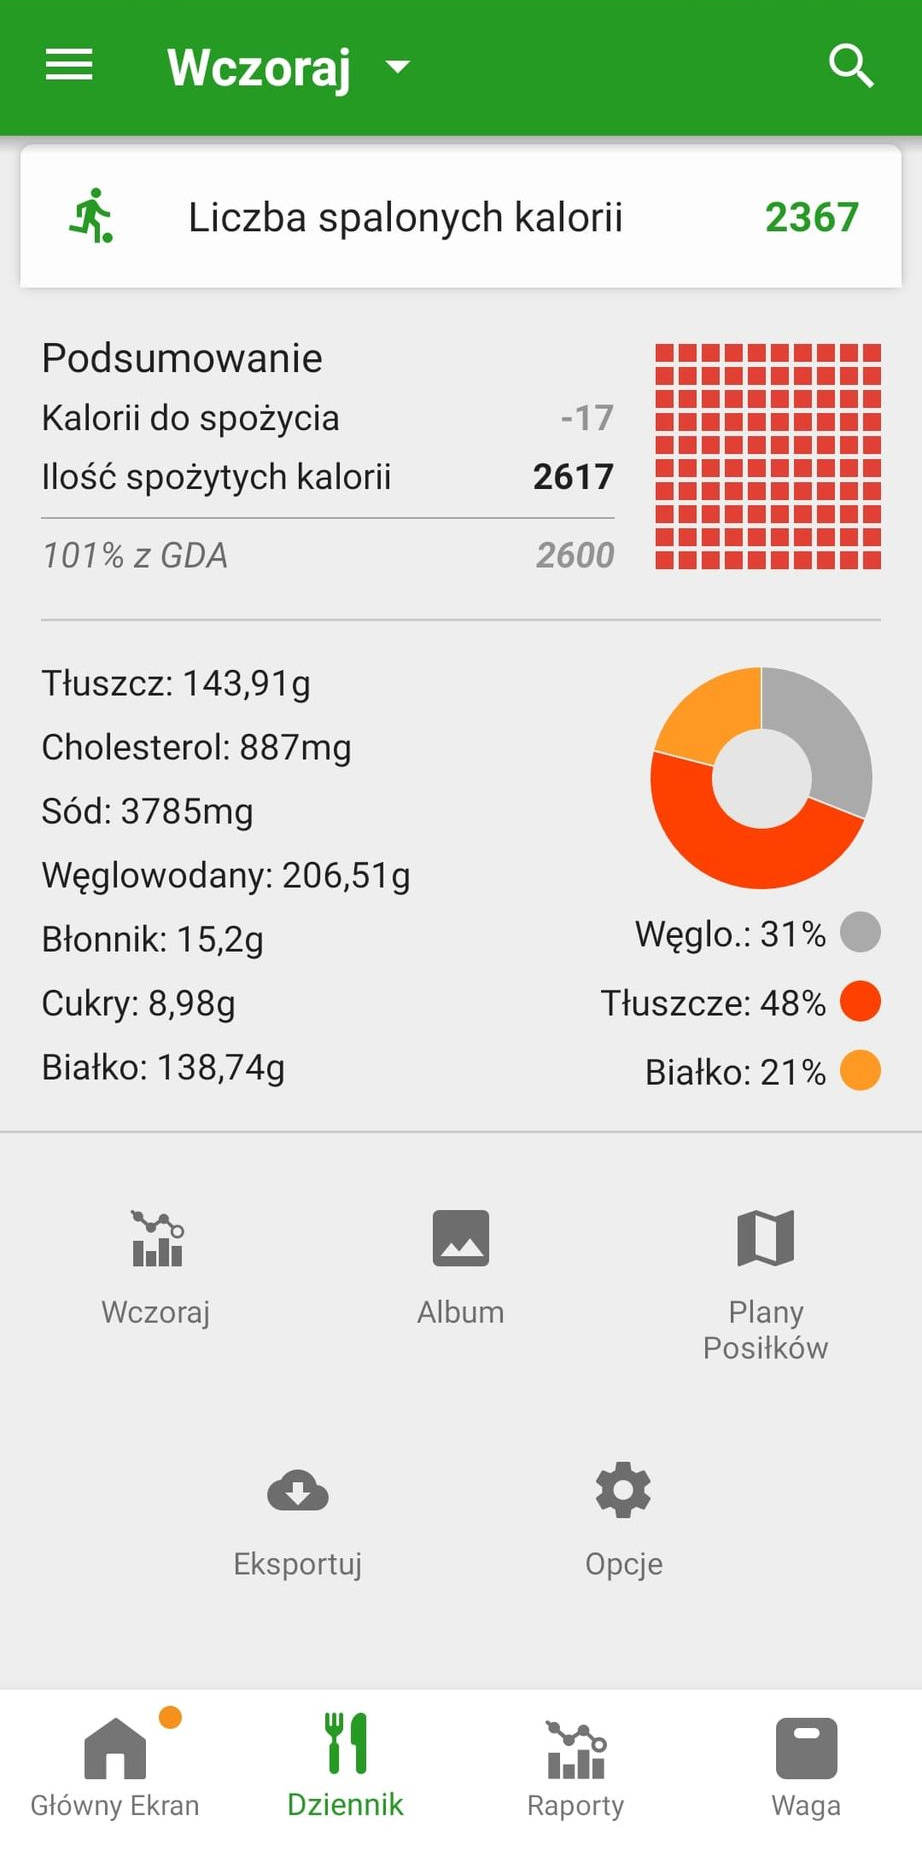
\includegraphics[width=.3\textwidth]{fatsecret_2.png}
        \caption{Fatsecret - Ekran podsumowujący}
        \label{fig:fat2}
      \end{figure}
      
      \begin{figure}[H]
        \centering
        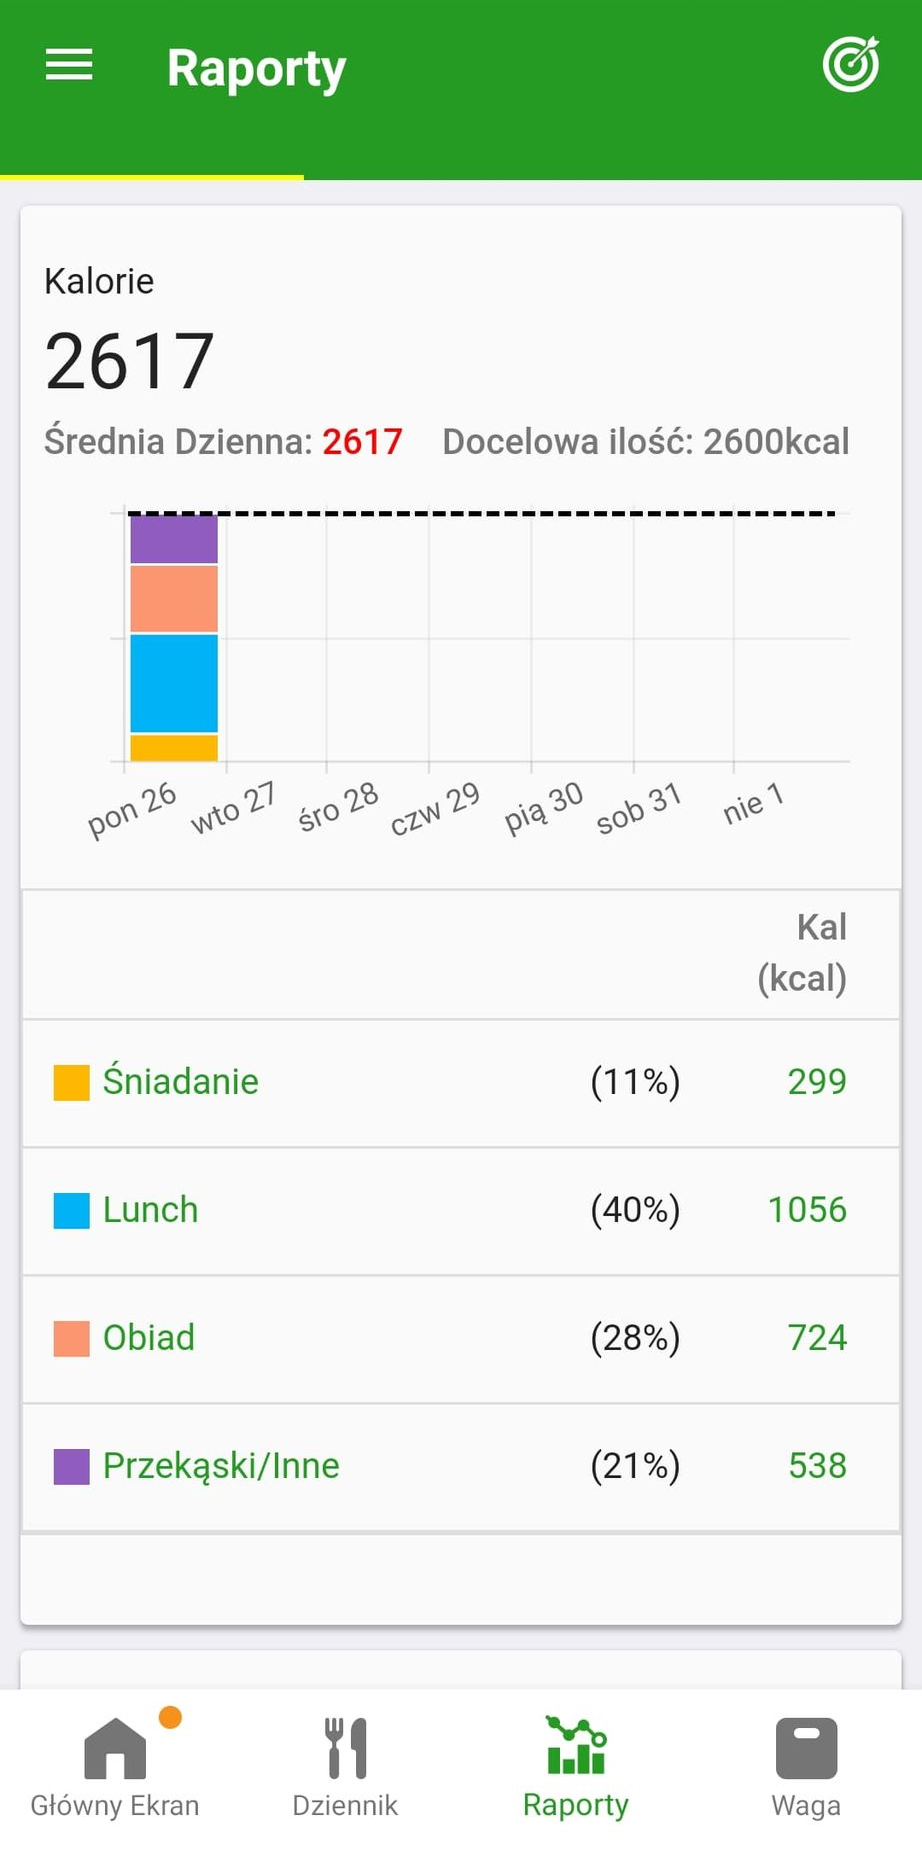
\includegraphics[width=.3\textwidth]{fatsecret_3.png}
        \caption{Fatsecret - Ekran raportu}
        \label{fig:fat3}
      \end{figure}
    }
  }
  \subsection{Wymagania funkcjonalne}
  {
    Wymagania funkcjonalne jest to grupa założeń, opisujących co ma realizować system, 
    jak ma się zachowywać w określonych sytuacjach, jakie usługi ma dostarczać i jaką ma
    pełnić funkcję.

    \begin{itemize}
      \item Formularz rejestracyjny powinien pozwolić w prosty i szybki sposób założyć 
      konto w aplikacji, co pozwala użytkownikowi przechowywać informacje w 
      chmurowej bazie danych.
      \item Panel logowania ma udostępniać formularz identyczny do panelu rejestracji,
      jednak pozwolić ma na uzyskanie dostępu do konta na które rejestrowane są
      zjedzone produkty.
      \item Zjedzone produkty mogą zostać dodane do listy na 2 sposoby:
        \begin{itemize}
          \item Przy pomocy pola tekstowego, poprzez wpisanie odpowiedniej frazy.
          \item Przy pomocy przytrzymania przycisku rozpoczynającego nasłuchiwanie telefonu.
          w celu rozpoznawania mowy. Aplikacja nie obsługuje wielu fraz wypowiedzianych
          jednocześnie, więc wyśle ona zapytanie do API żywnościowego załączając tylko 
          pierwsze wypowiedziane słowo.
        \end{itemize}
        Po dodaniu jedzenia, zostaje ono zapisane w bazie danych, a następnie można je
        wyświetlić po przejściu na ekran podsumowujący. Przy pomocy kalendarza,
        użytkownik ma także możliwość zmienić obecnie wyświetlany dzień, w celu
        sprawdzenia produktów spożytych w innej dacie.
      \item Całkowita ilość spożytych kalorii jest na bieżąco sumowana i wyświetlana na
      ekranie głównym. Wartość ta jest zmieniana w zależności od obecnie wyświetlanej daty. 
    \end{itemize}
  }
  \subsection{Wymagania niefunkcjonalne}
  {
    Wymagania niefunkcjonalne opisują ograniczenia, przy zachowaniu których system
    powinien realizować swoje zadania. Dotyczą przykładowo niezawodności, bezpieczeństwa,
    przenośności \cite{funk-niefunk}.

    \begin{itemize}
      \item Dane użytkownika mają być dostępne do odczytu tylko i wyłącznie dla niego, po 
      zalogowaniu na konto.
      \item W przypadku błędnie wpisanej frazy podczas wyszukiwania, aplikacja ma 
      zwrócić okno z tekstową wiadomością, informującą użytkownika o problemie przy
      znalezieniu produktu.
      \item Aplikacja powinna dostosować szatę graficzną do różnych rozdzielczości ekranu.
      \item Aplikacja nie powinna móc działać w tle i wykorzystywać zasoby.
      \item Aplikacja ma być zaprojektowana pod system operacyjny "Android".
      \item Aplikacja oczekuje dostępu do mikrofonu. 
      \item Aplikacja ma mieć prosty interfejs i pozwolić użytkownikowi na szybką naukę
      jej obsługi.
    \end{itemize}
  }
}

\section{Technologie i narzędzia wykorzystane w projekcie}
{

  \subsection{Dart}
  {
    Dart jest językiem programowania opracowanym przez firmę Google i pierwszy raz
    ukazanym na konferencji Aarhus w 2010 roku. Jego głównym celem było wprowadzenie
    konkurencji dla JavaScriptu, dominującego języka używanego w przeglądarkach
    internetowych. Cechuje go fakt, że jest językiem programowania obiektowego, opartym
    na klasach ze składnią podobną do języków z rodziny "C", a jego kod może zostać
    skompilowany na zarówno kod maszynowy, przy użyciu maszyny wirtualnej Dart VM, jak
    i przy pomocy kompilatora "dart2js", na kod JavaScript, co przekłada się na jego
    kompatybilność z wieloma obecnymi przeglądarkami internetowymi. Dart VM umożliwia
    łatwe uruchamianie kodu na różnych platformach, bez potrzeby pisania aplikacji pod
    konkretny system, a także oferuje dwa różne tryby kompilacji \cite{dart}:
    \begin{itemize}
      \item Just-in-time compiler (JIT) - pozwala na inkrementalną kompilację,
      umożliwiającą szybkie sprawdzenie wyniku wprowadzonych w kodzie zmian, z dostępem do
      wielu narzędzi służących debuggowaniu, bez potrzeby oczekiwania na całkowitą
      kompilację całego programu.
      \item Ahead-of-time compilation (AOT) - w momencie gdy aplikacja jest gotowa do
      wydania, Dart AOT umożliwia kompilację na kod maszynowy dla architektury ARM
      (używanej głównie w procesorach, lub urządzeniach mobilnych), bądź x86\_64
      (charakterystycznej dla komputerów stacjonarnych).
    \end{itemize}
    Dart wspiera pojedyncze dziedziczenie, gdzie klasa podrzędna może dziedziczyć tylko
    po jednej klasie nadrzędnej, interfejsy, domieszki, klasy abstrakcyjne, a także typy
    opcjonalne. O ile język ten wciąż nie zastąpił JavaScript na rynku aplikacji web'owych,
    tak zyskuje coraz większą popularność dzięki platformie programistycznej opracowanej
    przez Google, o nazwie "Flutter".
  }
  \subsection{Flutter}
  {
    Flutter jest względnie młodym frameworkiem, gdyż został pierwszy raz zaprezentowany
    w roku 2015 i miał początkowo służyć jako nowoczesna platforma do tworzenia aplikacji
    na system Android, a jego wersja alfa (0.0.6) została wydana w 2017 roku.
    Opracowany na bazie języka programistycznego Dart, Flutter skupia się
    na udostępnieniu narzędzi do szybkiego i łatwego projektowania interfejsu użytkownika,
    będąc przy tym bardzo wydajnym. Obecnie, umożliwia on używanie tego samego kodu na
    wielu platformach, takich jak Android, czy iOS, jako że w przeciwieństwie do
    konkurencyjnych rozwiązań, nie wykorzystuje on narzędzi oferowanych przez daną
    platformę \cite{flutter}. Zamiast tego, Flutter opiera się w pełni na własnym
    systemie "widget'ów", co pozwala wyróżnić go pod względem szybkości i wydajności,
    i tak jak w przypadku systemu Windows zwykło się mówić, że wszystko w Windows jest
    oknem, tak we Flutterze wszystko jest widgetem. Tworzą one wspólnie drzewo hierarchiczne,
    gdzie każdy widget dziedziczy po innym, nadrzędnym komponencie, aż do widgetu będącego
    kontenerem przechowującym całą aplikację, zwanego zazwyczaj MaterialApp, lub
    CupertinoApp.\\
    Sam framework Flutter'a jest relatywnie mały i ograniczony, a większość bardziej
    zaawansowanych komponentów jest udostępniana w formie pakietów i pluginów, które
    programiści w zależności od potrzeb mogą dowolnie załączać do swojego projektu.
  }
  \subsection{Cloud Firestore}
  {
    Cloud Firestore jest jedną z usług dostępnych w Google Firebase - platformy której
    głównym celem jest wspomaganie twórców aplikacji mobilnych poprzez oferowanie
    zestawu gotowych narzędzi. Firestore jest nierelacyjną, chmurową bazą danych, która
    jest w stanie w czasie rzeczywistym informować aplikację o zmianach w swojej bazie,
    co pozwala na ciągłe wyświetlanie najnowszych danych, bez potrzeby specjalnego,
    interwałowego ich sprawdzania. Posiada ona wsparcie dla trybu offline i w przypadku
    gdy urządzenie utraci dostęp do internetu, Cloud Firestore buforuje dane, z których
    aktywnie korzysta aplikacja, a następnie po odzyskaniu połączenia synchronizuje
    wszelkie lokalne zmiany z danymi znajdującymi się w chmurze.\\
    Dane w Firestore przechowywane są zgodnie z modelem danych NoSQL, w dokumentach
    zawierających pola mapowane na wartości. Te dokumenty przechowywane są w kolekcjach - \\
    kontenerach na dokumenty, których można używać do organizowania danych i tworzenia
    zapytań. Dokumenty są w stanie obsłużyć wiele różnych typów danych, od prostych
    łańcuchów i liczb po złożone, zagnieżdżone obiekty. Ponadto, dane mogą być odczytywane
    na poziomie dokumentu, bez konieczności pobierania całej kolekcji lub jakichkolwiek
    zagnieżdżonych podkolekcji.
  }
  \subsection{Android Studio}
  {
    Android Studio jest oficjalnym narzędziem do tworzenia aplikacji na system operacyjny
    "Android", opartym na środowiskach programistycznych firmy IntelliJ i oprócz
    standardowego zestawu narzędzi i edytora kodu, oferuje szereg ułatwień z myślą
    o aplikacjach mobilnych. Jako fundacji do budowania rozwiązania, Android Studio używa
    "Gradle", uznanego oprogramowania open-source służącego do automatyzacji całego procesu.
    Do łatwego testowania aplikacji, Android Studio posiada wbudowany emulator, pozwalający
    na ściągnięcie dowolnej, pożądanej wersji systemu operacyjnego, na telefony o
    różnych rozmiarach ekranu. Środowisko oferuje również wsparcie dla systemu kontroli
    wersji "Git", stąd proces zapisania wszelkich zmian i wysłania ich na repozytorium
    może zostać w pełni wykonany przy pomocy Android Studio.
  }
  \subsection{Android Emulator}
  {
    Do aktywnego sprawdzania aplikacji mobilnych na desktopach, używa się
    specjalnych emulatorów, których zadaniem jest stworzenie wirtualnego środowiska
    przypominającego w działaniu realne urządzenie przenośne, poprzez naśladowanie
    sprzętu znajdującego się w urządzeniach mobilnych. Odzwierciedlenie realnego
    procesora byłoby zadaniem wyjątkowo wymagającym pod względem zasobów,
    przekładając się na szybkość z jaką działałby dany emulator, jednak dzięki wspomnianemu
    wcześniej w przypadku maszyn wirtualnych oprogramowaniu "Hypervisor", gdy architektury
    procesorów urządzenia emulowanego jak i komputera stacjonarnego są ze sobą zgodne,
    możliwe jest użycie procesora hosta, jako procesora w emulowanym urządzeniu.\\
    Największą zaletą używania emulatorów jest oczywiście prędkość, z jaką można testować
    swoją aplikację, bez zbędnej potrzeby budowania jej, a następnie eksportowania
    na posiadane urządzenie mobilne, instalowania, a w końcu sprawdzania. Inną mniej
    oczywistą, jest testowanie aplikacji pod kątem interakcji z fizycznymi
    sensorami, jak przykładowo akcelerometr, gdyż dużo łatwiej jest dostosować ustawienia
    w wirtualnym środowisku, aby następnie mogły one poprawnie działać już na realnym
    urządzeniu.\\
    Wraz z zaletami pojawiają się także ograniczenia. Najpopularniejszą architekturą
    dla urządzeń mobilnych jest ARM v7a, jednak większość desktopów używa x86\_64, stąd
    bez procesora z architekturą ARM w większości przypadków nie ma nawet okazji skorzystać
    z przyspieszonej emulacji, wspomnianej wcześniej. Stworzenie jednego wirtualnego
    urządzenia może zająć nawet do 10GB miejsca na dysku, stąd posiadanie wielu różnych
    urządzeń do testowania w znacznym stopniu ogranicza dostępną pamięć systemową.
    Wydajność z jaką operuje emulator jest ściśle związana z urządzeniem na którym jest
    on uruchomiony, stąd może on nie tylko działać wolniej niż zazwyczaj, ale także
    wyrzucać błędy, niekoniecznie związane z działaniem samej aplikacji, lub emulatora.\\
    Emulatory nigdy nie będą w stanie w pełni oddać działania prawdziwego urządzenia i
    nie będą w stanie zaoferować wszystkich dostępnych w urządzeniach mobilnych możliwości,
    także testowanie na fizycznym urządzeniu zawsze będzie procederem wymaganym, do
    prawidłowego projektowania aplikacji mobilnych.
  }
  \subsection{VIM}
  {
    VIM jest zaawansowanym edytorem tekstu opracowanym w 1991 roku, opartym na edytorze
    "vi", domyślnie dołączanym do większości systemów UNIX. Jest dystrybuowany jako
    "charityware" - dostęp do niego jest darmowy, ale twórca zachęca do wpłaty pieniędzy
    na cele charytatywne. VIM charakteryzuje szeroki wachlarz możliwości jakie oferuje,
    a w odpowiednich rękach pozwala bardzo zwiększyć wydajność pracy. Używanie VIMa
    nie wymaga myszki, jego głównym celem jest ograniczenie konieczności poruszania ręką
    pomiędzy klawiaturą, a myszką, na rzecz wykonywania każdej czynności przy takim samym
    ustawieniu rąk. Wraz z rozwojem aplikacji, stale dodawane są nowe funkcjonalności,
    mające w jeszcze większym stopniu usprawnić proces pisania. VIM zezwala na
    modyfikowanie i dodawanie własnych skrótów klawiszowych, oraz posiada wiele opcji
    konfiguracji, stąd zależnie od preferencji i potrzeb można go dostosować do wielu
    postaci.\\
    Do podstawowych opcji udostępnianych przez VIM należą:
    \begin{itemize}
      \item do poruszania się kursorem służą klawisze:
      \begin{itemize}
        \item h - jeden znak w lewo
        \item j - linijka w dół
        \item k - linijka w górę
        \item l - jeden znak w prawo
        \item b - poprzednie słowo
        \item e - koniec słowa
        \item w - początek następnego słowa
        \item \$ - koniec linii 
        \item 0 - początek linii
      \end{itemize}
      \item do przełączania się pomiędzy różnymi trybami służą klawisze:
      \begin{itemize}
        \item i - Insert mode, włączający możliwość pisania po lewo od kursora
        \item a - Insert mode, włączający możliwość pisania po prawo od kursora
        \item o - Insert mode, włączający możliwość pisania o jedną linię niżej
        \item v - Visual mode, pozwalający zaznaczyć część tekstu
        \item ESC - umożliwia przejście do Normal mode, domyślnego trybu poruszania się
        \item : - włączenie trybu Command-line, umożliwiającego dostęp nie tylko do
        zaawansowanych opcji, ale także opcji zapisu lub wyjścia z pliku
      \end{itemize} 
    \end{itemize}
    Przedstawione wyżej opcje to tylko wierzchołek góry lodowej, a poprawne nauczenie
    się możliwości oferowanych przez VIM może zająć wiele miesięcy.
  }
}

\section{Proces powstawania aplikacji}
{
}

\section{Podsumowanie}
{
}

\section{Indeks rysunków}

\section{Bibliografia}
{
  \printbibliography
  %https://www.oracle.com/pl/database/what-is-database/#link5
  %https://smartbees.pl/blog/co-jest-api-wszystko-o-interfejsie-programowania-aplikacji
  %https://www.cdc.gov/nchs/products/databriefs/db360.htm
  %https://runrepeat.com/gym-membership-statistics
  %https://fs.siteor.com/ecdl/files/RODZAJE_BAZ_DANYCH_I_ICH_BUDOWA.pdf?1289369360
}

\end{sloppypar}
\end{document}